
\documentclass[11pt]{article}

% Packages

\usepackage[czech]{babel}
\usepackage[utf8]{inputenc}
\usepackage[useregional]{datetime2}
\usepackage[T1]{fontenc}
\usepackage[a4paper, total={15.24cm, 23.32cm}]{geometry}
\usepackage[thinlines]{easytable}
\usepackage{graphicx}
\usepackage[ampersand]{easylist}
\usepackage{changepage}
\usepackage{float}
\usepackage{color}
\usepackage{siunitx}
\usepackage{hyperref}
\usepackage{amssymb}
\usepackage{amsmath}
\usepackage{amsfonts}
\usepackage{enumitem}
\usepackage{mathtools}
\usepackage{calc}
\usepackage{wrapfig}

% Config
%\setlength\parindent{0pt}
\renewcommand{\baselinestretch}{1.2} 
\setitemize{itemsep=0pt}
\hypersetup{
	colorlinks,
	citecolor=black,
	filecolor=black,
	linkcolor=black,
	urlcolor=black
}
\title{\textbf{V. Počítačová grafika a analýza obrazu}}
\date{\small\vspace{-9ex}Update: \today}
\DeclareUnicodeCharacter{2212}{-}
\DeclareUnicodeCharacter{200B}{ }
\begin{document}
\maketitle
\setcounter{tocdepth}{1}
\tableofcontents
\pagebreak

\section{Osvětlovací modely a systémy barev v počítačové grafice.}
\subsection{Architektura mikroprocesorů}
\textbf{Architektura procesoru} je náčrt struktury a funkčnosti systému. Je charakterizována výčtem \textbf{registrů} a jejich funkcí, vnitřních a vnějších \textbf{sběrnic}, způsobem \textbf{adresování} a \textbf{instrukčním souborem}.

\textbf{Registr} je malé úložiště dat v mikroprocesoru s rychlým přístupem, které slouží jako \textbf{pracovní paměť} během výpočtů.

\textbf{Sběrnice} je soustava vodičů pro \textbf{přenos informací} mezi více účastníky na principu \uv{jeden vysílá, ostatní přijímájí.} Podle typu přenášené informace je dělíme na \textit{datové}, \textit{adresové} a \textit{řídící}. V praxi však díky multiplexu může jít o jedny dráty.

\subsection{Procesory CISC a RISC}
V dnešní době se ustálilo dělení počítačů do dvou základních kategorií podle typu používaného procesoru:
\begin{itemize}
	\item{\textbf{CISC} -- počítač se složitým souborem instrukcí (\textit{Complex Instruction Set Computer})}
	\item{\textbf{RISC} -- počítač s redukovaným souborem instrukcí (\textit{Reduced Instruction Set Computer})}
\end{itemize}

\subsubsection{CISC}
\begin{itemize}
	\item Procesory s \textbf{komplexním instrukčním souborem}.
	\item Instrukce mají \textbf{proměnlivou délku} i \textbf{dobu vykonání}.
	\item \textbf{Vysoká složitost instrukcí} $\,\to\,$ nutný systematický návrh řadiče procesoru.
	\item Vykonání strojové instrukce probíhá posloupností mikrooperací (předepsána mikroinstrukcí v řídící paměti).
	\item Procesor obsahuje relativně \textbf{nízký počet registrů}.
	\item Operace provedená i \textbf{složenou instrukcí} (např. násobení) může být \textbf{nahrazena} sledem jednodušších strojových instrukcí (\textit{sčítání a bitové posuny}) $\,\to\,$ mohou být ve výsledu vykonány rychleji, než hardwarově implementovaná složená varianta.
	\item {Označení \textbf{CISC} bylo zavedeno jako \textbf{protiklad} až poté, co se prosadily procesory RISC, které mají instruční sadu naopak maximálně redukovanou (pouze jednoduché operace, tj. žádné složené, jsou stejně dlouhé a jejich vykonání trvá stejnou dobu).}
	\item {Obvyklou chybou je domněnka, že procesory CISC mají více strojových instrukcí, než procesory RISC. Ve skutečnosti nejde o absolutní počet, ale o \textbf{počet různých druhů operací}, které procesor sám přímo umí vykonat na hardwarové úrovni (tj. již z výroby). Procesor CISC tak může například paradoxně obsahovat jen jednu strojovou instrukci pro danou operaci (např. \textit{logické operace}), zatímco procesor RISC může tuto operaci obsahovat jako několik strojových instrukcí, které stejnou operaci umí provést nad různými registry.}
\end{itemize}
\begin{figure}[H]
\centering
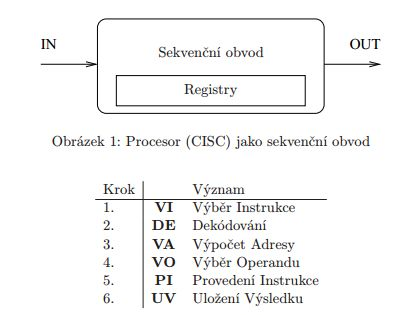
\includegraphics[width=0.6\textwidth]{assets/1_cisc_sekv}
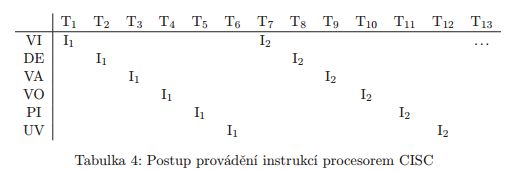
\includegraphics[width=0.6\textwidth]{assets/1_cisc_instrukce}
\end{figure}

\subsubsection{RISC}
\begin{itemize}
\item {\textbf{Počet instrukcí a způsobů adresování je malý, ale zůstává úplný}, aby bylo možno provést vše $\,\to\,$ v tomhle se liší od CISC}.
\item {Instrukce jsou vytvořeny pomocí obvodu $\,\to\,$ jednodušší na výrobu než CISC}.
\item Je menší počet instrukcí, takže složitější instrukce se nahradí větším počtem jednodušších.
\item To způsobuje nárust kódu. Zároveň ale vznikly rychlejší sběrnice, tj rychlejší proud dat do procesoru.
\item {Používá se \textbf{zřetězené zpracování instrukcí} (Blíže popsáno níže)}. 
\item {Instrukce se provádějí jen nad registry}.
\item {Navýšený počet registrů $\,\to\,$ delší program}.
\item {Instrukce mají \textbf{jednotný formát} -- délku i obsah}.
\item {Komunikace s pamětí pouze pomocí instrukcí \textbf{LOAD / STORE}, adresování i práce je celkově rychlejší}.
\item V návaznosti je využívaná cache pro co nejrychlejší přístup dat.
\item Využívá se \textbf{predikce skoků}, takže se začnou načítat data, která pravděpodobně budou v další instrukci potřeba.
\item {\textbf{Každý strojový cyklus znamená dokončení jedné instrukce}}.
\item {Řešení problémů s frontou instrukcí}.
\item {Mikroprogramový řadič může být nahrazen rychlejším obvodem}.
\item {Představitelé \textbf{ARM, MOTOROLA 6800, INTEL i960, MIPS R6000}}.
\end{itemize}
\begin{figure}[H]
\centering
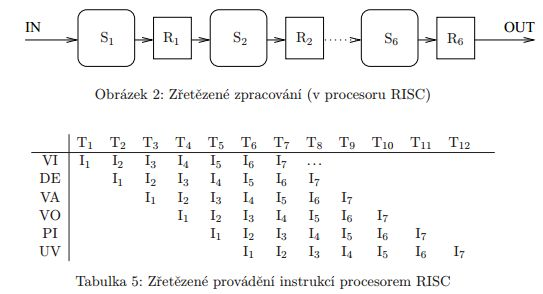
\includegraphics[width=0.6\textwidth]{assets/1_risc_zretezeni}
\end{figure}

\subsection{Von Neumannovo schéma počítače}

John Von Neumann definoval v roce \textbf{1945} základní koncepci počítače (EDVAC) \textbf{řízeného obsahem paměti}. Od té doby se objevilo několik odlišných modifikací, ale v podstatě se \textbf{počítače v dnešní době} konstruují podle tohoto modelu. Ve svém projektu si von Neumann stanovil určitá kritéria a principy, které musí počítač splňovat, aby byl použitelný univerzálně. Můžeme je ve stručnosti shrnout do následujících bodů:
\begin{itemize}
\item Počítač se skládá z paměti, řídící jednotky, aritmeticko--logické jednotky, vstupní a  výstupní jednotky.
\begin{enumerate}
\item \textbf{ALU} -- aritmeticko-logická jednotka (aritmetic-logic unit) => jednotka provádějící veškeré aritmetické výpočty a logické operace. Obsahuje sčítačky, násobičky a komparátory.
\item  \textbf{Operační paměť} -- slouží k uchování zpracovávaného programu, zpracovávaných dat a výsledků výpočtu.
\item \textbf{Řídící jednotka} -- řídí činnost všech částí počítače. Toto řízení je prováděno pomocí řídících signálů, které jsou zasílány jednotlivým modulům. Řadiči jsou pak zpět zasílané stavové hlášení. Dnes řadič spolu s ALU tvoří jednu součástku, a to procesor neboli CPU (Central Processing Unit).
\item \textbf{Vstup/Výstup} -- zařízení určené pro vstup dat, a výstup zpracovaných výsledků.
\end{enumerate}
\item Struktura pc je \textbf{nezávislá na typu řešené úlohy} (univerzálnost), \textbf{počítač se programuje obsahem paměti}.
\item Následující krok počítače je závislý na kroku předešlém.
\item \textbf{Instrukce} a \textbf{data} jsou v téže paměti.
\item Paměť je rozdělena do \textbf{paměťových buněk stejné velikosti (Byte)}, jejichž pořadová čísla se využívají jako adresy.
\item Program je tvořen posloupností instrukcí, které se vykonávají jednotlivě v pořadí, v jakém jsou zapsány do paměti.
\item Změna pořadí prováděných instrukcí se provádí \textbf{skokovými instrukcemi} (podmíněné nebo nepodmíněné skákání na adresy). 
\item Čísla, instrukce, adresy a znaky se značí v \textbf{binární soustavě}.
\end{itemize}
\begin{figure}[H]
\centering
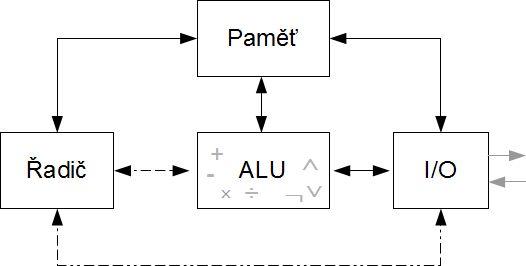
\includegraphics[width=0.6\textwidth]{assets/1_vonNeumann}
\end{figure}

\subsubsection{Nevýhody Von Neumannovy koncepce ve srovnání s dnešními PC}
\begin{itemize}
\item Podle von Neumannova schématu počítač pracuje \textbf{vždy nad jedním programem}. Toto vede k velmi špatnému využití strojového času. Dnes je obvyklé, že počítač \textbf{zpracovává paralelně více programů} zároveň - tzv. \textbf{multitasking}.
\item Počítač může mít i více jak jeden procesor.
\item Podle Von Neumanova schématu mohl počítač pracovat pouze v tzv. \textbf{diskrétním režimu}, kdy byl do paměti počítače zaveden program, data a pak probíhal výpočet. V průběhu výpočtu již nebylo možné s počítačem dále interaktivně komunikovat.
\item Dnes existují \textbf{vstupní/výstupní} zařízení, např. pevné disky a páskové mechaniky, které umožňují vstup i výstup.
\item Program se do paměti nemusí zavést celý, ale je možné zavést pouze jeho část a ostatní části zavádět až v případě potřeby.
\end{itemize}

\noindent\makebox[\textwidth]{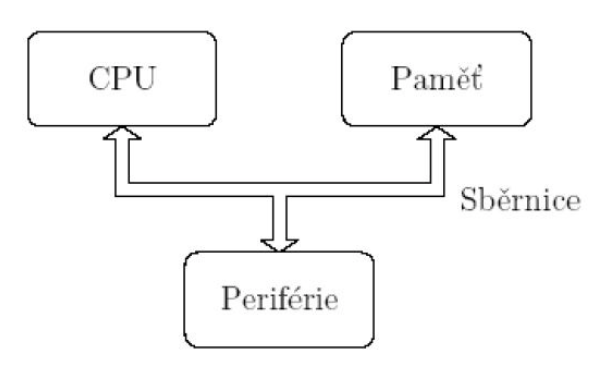
\includegraphics[width=8cm]{assets/1_neuman2}}

\subsubsection*{Výhody}
\begin{itemize}
	\item[$+$] \textbf{Rozdělení paměti} pro kód a data určuje programátor, řídící jednotka přistupuje pro  data i instrukce jednotným způsobem.
	\item[$+$] \textbf{Jedna sběrnice} ->  jednodušší levnější výroba.
\end{itemize}
\subsubsection*{Nevýhody}
\begin{itemize}
	\item[$-$] \textbf{Společné uložení dat a kódu} může mít za následek přepsání vlastního programu.
	
	\item[$-$] \textbf{Jedna sběrnice} je omezující.
\end{itemize}

\subsection{Hardvardské schéma počítače}
Několik let po von Neumannovi, přišel vývojový tým odborníků z Harvardské univerzity s vlastní koncepcí počítače, která se sice od Neumannovy příliš nelišila, ale odstraňovala některé její nedostatky. V podstatě jde pouze o \textbf{oddělení paměti pro data a program}. Abychom si mohli obě koncepce porovnat, můžeme vycházet ze zjednodušených schémat.
\newline

\noindent\makebox[\textwidth]{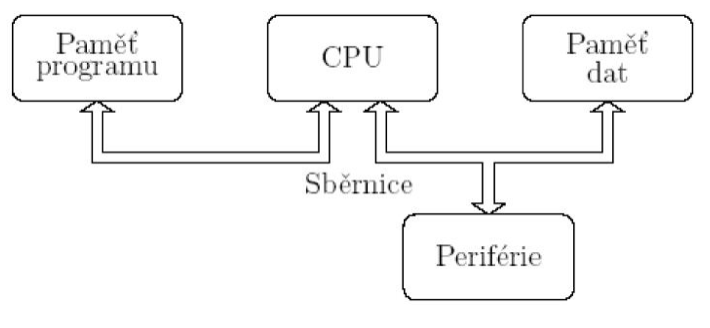
\includegraphics[width=8cm]{assets/1_harvard}}

\subsubsection*{Výhody}
\begin{itemize}
	\item[$+$]\textbf{Program se nepřepíše} (oddělené paměti pro data a program).
	\item[$+$]Dvě sběrnice umožňují \textbf{paralelní} načítání instrukcí a dat.
	\item[$+$]Paměti mohou být vyrobeny \textbf{odlišnými technologiemi }a každá může mít jinou nejmenší adresovací jednotku (8 bitů pro instrukce a 8, 16 nebo 32 pro data).
\end{itemize}


\subsubsection*{Nevýhody}
\begin{itemize}
\item[$-$]2 sběrnice mají \textbf{vyšší nároky na vývoj} řídící jednotky a jsou také dražší a složitější na výrobu.
\item[$-$]Paměť je \textbf{rozdělena} už od \textbf{výrobce}.
\item[$-$]Nevyužitou část dat \textbf{nelze využít }po program a obráceně.
\end{itemize}

\pagebreak
\subsection{Principy urychlování činnosti procesorů}
\begin{itemize}
	\item{Speciální kódování dle potřeby dané úlohy}.
	\item{Speciální výpočetní jednotky dle potřeby dané úlohy (FFT -- rychlá fourierova transformace)}.
	\item{Paralelní zpracování (násobné výpočetní jednotky)}.
	\item{\textbf{Zřetězové zpracování instrukcí} (pipelining)}.
	\item{Využití cache pamětí (L1, L2, L3)}.
	\item{Predikce skoků}
\end{itemize}
\subsubsection{Paralelní zpracování}
Zpracování více elementárních úloh běží součastně.
\begin{figure}[H]
\centering
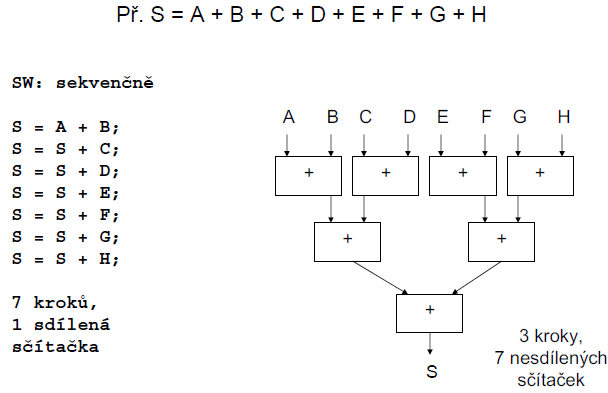
\includegraphics[width=0.6\textwidth]{assets/1_paralelni_zpracovani.png}
\end{figure}

\subsubsection{Zřetězené zpracování instrukcí (pipelining)}
Princip zřetězení se značně překrývá s principy procesorů RISC.
%\subsection{Problémy zřetězeného zpracování}
 Základní myšlenkou je \textbf{rozdělení zpracování jedné instrukce} mezi různé části procesoru a tím i dosažení možnosti \textbf{zpracovávat} \textbf{více instrukcí }najednou. Pro dosažení tohoto zřetězení je nutné rozdělit úlohu do posloupnosti dílčích úloh, z nichž každá může být vykonána \textbf{samostatně}, např. oddělit načítaní a ukládání dat z paměti od provádění výpočtu instrukce a tyto části pak mohou běžet souběžně. To znamená že musíme osamostatnit jednotlivé části sekvenčního obvodu tak, aby každému obvodu odpovídala jedna fáze zpracování instrukcí. Všechny fáze musí být \textbf{stejně časově náročné}, jinak je rychlost \textbf{degradována} na nejpomalejší z nich. Fáze zpracování je rozdělena minimálně na 2 úseky:
\begin{itemize}
\item \textbf{Načtení} a \textbf{dekódování} instrukce.
\item \textbf{Provedení} instrukce a případné uložení výsledku.
\end{itemize}
Zřetězení se stále vylepšuje a u novějších procesorů se již můžeme setkat stále s více řetězci rozpracovaných informací (více pipelines), dnes je standardem 5 pipelines.

\subsubsection{Problém a predikce skoků}
Největší problém spočívá v \textbf{plnění zřetězené jednotky}, hlavně při provádění \textbf{podmíněných skoků}, kdy během stejného počtu cyklů se vykoná více instrukcí. U pipelingu se instrukce následující po skoku vyzvedává dřív, než je skok dokončen. \textbf{Primitivní implementace} vyzvedává vždy \textbf{následující instrukci}, což vede k tomu, že se vždy mýlí, pokud je skok nepodmíněný. Pozdější implementace mají \textbf{jednotku předpovídání skoku (1bit)}, která vždy správně \textbf{předpoví nepodmíněný skok} a s použitím cache se záznamem předchozího chování programu se pokusí předpovědět i cíl podmíněných skoků nebo skoků s adresou v registru nebo paměť. V případě, že se predikce nepovede, bývá nutné vyprázdnit celou pipeline a začít vyzvedávat instrukce ze správné adresy, což znamená relativně \textbf{velké zdržení}. Související problémem je přerušení.

\subsubsection{Plnění fronty instrukcí}
Pokud se dokončí skoková instrukce, která odkazuje na jinou část kódu, musejí být instrukce za ní zahozeny (\textit{problém plnění fronty instrukcí}).
\begin{itemize}
	\item{U malého zřetězení \textbf{neřešíme}}.
	\item{Používání bublin na vyprázdnění pipeline, \textbf{naplněníní prázdnými instrukcemi}}.
	\item{\textbf{Predikce skoku} -- vyhrazen jeden bit předurčující, zda se skok provede či nikoliv}.
\end{itemize}
\begin{itemize}
	\item{\textbf{Statická} -- součást instrukce $\,\to\,$ řeší programátor nebo kompilátor}
	\item{\textbf{Dynamická} 
			\begin{itemize}
					\item{\textbf{jednobitová} -- zaznamenává jestli se skok provedl, či ne (1/ 0)}
					\item{\textbf{dvoubitová} -- metoda zpožděného skoku $\,\to\,$ v procesoru řeší se např. tabulkou s 4 kB instrukcí}
			\end{itemize}
		}
\end{itemize}
Zřetězené zpracování přináší urychlení výpočtu nejen v procesorech, ale i jiných číslicových obvodech (např. pro zpracování obrazu, bioinformatických dat apod.). Pokud použijeme zřetězené zpracování, musíme dodat řadu podpůrných obvodů a řešit řadu nových problémů. \textbf{Moderní procesory používají kromě zřetězení i další koncepty}:
\begin{itemize}
	\item{\textbf{Superskalární architektura} (zdvojení) -- když nastane podmíněný skok, začnou se vykonávat instrukce obou variant, nepotřebná část se pak zahodí. Tento způsob, pak vyžaduje vyřešit ukládání výsledku.}
	\item{\textbf{VLIW procesory} (Very long instruction word) -- umožňuje instrukční paralelismus (vykonávání několik nezávislých instrukcí souběžně), velmi dlouhé instrukční pakety}.
	\item{\textbf{Vektorové procesory} -- je navržený tak, aby dokázal vykonávat matematické operace nad celou množinou čísel v daném čase. Je opakem skalárního procesoru, který vykonává jednu operaci s jedním číslem v daném čase. }
	\item{\textbf{Vícevláknové procesory} }
\end{itemize}

\pagebreak	
\section{Afinní a projektivní prostor. Afinní a projektivní transformace a jejich matematický zápis. Aplikace v počítačové grafice. Modelovací a zobrazovací transformace.}
\subsection{Specifikace požadavků}
Specifikace a analýza požadavků je první fáze vývoje softwaru. \textbf{Cílem je definovat požadavky na software a popsat jeho funkcionalitu}. Výsledkem této fáze by měly být dokumenty, které se stanou součásti smlouvy mezi zadavatelem a vývojovým týmem. \textbf{Kvalita} výsledného produktu je pak dána \textbf{mírou uspokojení požadavků zadavatele}.

V rámci specifikace požadavků je třeba analyzovat procesy u zadavatele, které bude software řešit, nebo s ním nějak jinak souvisí. K popisu těchto procesů dobře poslouží \textbf{Diagram případu užití}, \textbf{Sekvenční diagram} a \textbf{Diagram aktivit}.

\subsubsection{Cíle požadavků}
\begin{itemize}
\item chceme vytvořit a udržovat dohody se zákazníky a dalšími zainteresovanými stranami o tom, co by \textbf{systém měl dělat a proč},
\item aby vývojáři lépe pochopili \textbf{požadavky na systém},
\item definování \textbf{hranic systému},
\item vytvořit základ pro plánování \textbf{technického obsahu} interakcí,
\item poskytnout základ pro \textbf{odhad} \textbf{nákladů} a \textbf{času} na \textbf{vytvoření systému},
\item definovat \textbf{uživatelské rozhraní} pro systém, se zaměřením na potřeby uživatelů.
\end{itemize}

\subsubsection{Aktivity spojené s analýzou požadavků}
\begin{itemize}
	\item \textbf{Sběr požadavků} --  komunikace se zákazníky a uživateli za účelem získání jejich požadavků na systém.
	\item \textbf{Analýza požadavků} -- identifikování nejasných požadavků, nekompletních, nebo protichůdných a následné řešení těchto nesrovnalostí.
	\item \textbf{Zaznamenání požadavků} -- dokumentování požadavků v různých formách, jako běžný textový dokument, případy užití (use case), nebo specifikace procesů.
\end{itemize}
Požadavky je také nutno: \textbf{organizovat}, \textbf{dokumentovat}, \textbf{priorizovat}, \textbf{filtrovat} a \textbf{sledovat}.

\subsubsection{Typy požadavků -- FURPS}
\begin{itemize}
\item \textbf{Funkční požadavky (chování)} -- se používají k vyjádření chování systému zadáním jak vstupních tak i výstupních podmínek.
\item \textbf{Doplňující požadavky (nefunkční)}
\begin{itemize}
\item \textbf{Použitelnost (Usability)} -- se zabývá lidskými faktory, jako je vzhled, snadné používání, atd.
\item \textbf{Spolehlivost (Reliability)} --  četnost a závažnost selhání, obnovitelnost a přesnost.
\item \textbf{Výkon (Performance)} -- se zabývá množstvím transakcí, jako je rychlost, doba odezvy, atd.
\item \textbf{Podporovatelnost (Supportability)} -- řeší, jak těžké je udržet systém a další vlastnosti potřebné k udržení systému po jeho vydání.
\end{itemize}
\end{itemize}

\subsection{Diagram případů užití}
\textbf{Případ užití (use case)} -- je technika pro zdokumentování případného požadavku na nový systém, nebo změny na stávající systém. Každý use case poskytuje jeden nebo více scénářů, které zaznamenávají, jak by systém měl spolupracovat s koncovým uživatelem nebo jiným systémem.

Diagram případu užití popisuje \textbf{vztahy} mezi \textbf{aktéry} a jednotlivými \textbf{případy užití}. Součástí diagramu jsou:
\begin{itemize}
\item \textbf{Aktéři} -- definují \textbf{uživatele} či \textbf{jiné systémy}, kteří budou vstupovat do interakce s vyvíjeným softwarovým systémem.
\item \textbf{Relace (vztahy)} -- \textbf{vazby} a \textbf{vztahy} mezi aktéry a případy užití. V diagramu jsou znázorněny \textbf{šipkami případně čárami}.
\item \textbf{Případy užití} -- specifikující vzory chování  softwarovým systémem.  Každý případ užití lze chápat jako \textbf{posloupnost vzájemně navazujících transakcí} vykonaných \textbf{v dialogu mezi aktérem a vlastním softwarovým systémem}.
\item \textbf{Scénář} -- unikátní sekvence akcí skrz use-case (jedna cesta/instance provedení).
\end{itemize}
\textbf{Účelem} diagramu případů užití \textbf{je definovat co existuje vně vyvíjeného systému} (\textbf{aktéři}) a \textbf{co má být systémem prováděno (případy užití)}. Vstupem pro sestavení diagramu případů užití je \textbf{byznys model}, konkrétně modely podnikových procesů.  \textbf{Výsledkem} analýzy těchto procesů \textbf{je seznam požadovaných funkcí softwarového systému}, které podpoří nebo dokonce nahradí některé z uvedených aktivity jejich softwarovou implementací.

\begin{figure}[H]
	\centering
	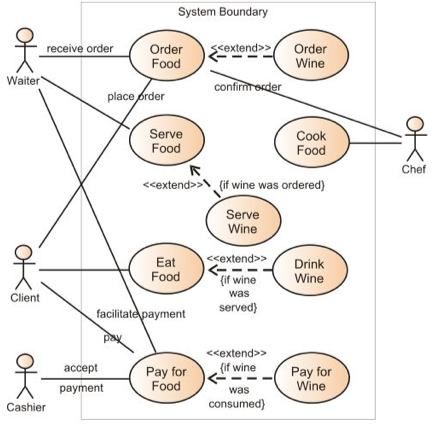
\includegraphics[width=0.7\textwidth]{assets/usecase.png}
\end{figure}

\noindent Pro složitější a obsáhlejší diagramy případů užití se zavadí \textbf{tři (+1) typy vztahů}:
\begin{itemize}
    \item \textbf{Relace} - bez typu (jen čára) značí přístup k UC, nejčastěji mezi aktéri a UC
\item \textbf{Include} – případ užití musí \textbf{obsahovat} jiný (UC s include se vždy provede před samotným UC).
\item \textbf{Extend} – případ užití může \textbf{rozšiřovat} jiný (UC s extend se může nebo nemusí provést).
\item \textbf{Generalizace} – případ užití může být \textbf{speciálním případem} jiného (dědičnost).
\end{itemize}

\subsubsection{Doporučená forma vytváření use-case}
\begin{itemize}
\item má vyjadřovat \textbf{co systém dělá} (ne jak) a co od něj očekávají aktéři,
\item měly by být používány jen pojmy problémové domény -- žádné neznámé termíny,
\item případy užití by měly být co \textbf{nejjednodušší}, ať jim rozumí i zadavatelé -- nepoužívat příliš \texttt{<include>} a \texttt{<extend>},
\item \textbf{nepoužívat} příliš funkční dekompozici (\textbf{specializaci}),
\item primární aktéři umístěni vlevo a pojmenováni krátkým podstatným jménem,
\item každý \textbf{aktér} by měl být \textbf{propojen s minimálně jedním use-case},
\item základní use case vlevo a další kreslit směrem doprava, rozšířující use-case směrem dolů.
\end{itemize}

\subsection{Sekvenční diagram}
Sekvenční diagram popisuje funkce systému z pohledu \textbf{objektů} a\textbf{ jejich interakcí}. Komunikace mezi objekty je \textbf{znázorněná v čase}, takže z diagramu můžeme vyčíst i životní cyklus objektu. 

Tento diagram popisuje jaké \textbf{zprávy} (\textbf{požadavky}) \textbf{jsou mezi objekty zasílány} \textbf{z pohledu času}. Diagram je tvořen \textbf{objekty uspořádanými do sloupců} a šipky mezi nimi odpovídají {vzájemně si zasílaným zprávám}. Zprávy mohou být {synchronní} nebo {asynchronní}. V případě \textbf{synchronních zpráv odesílatel čeká na odpověď} (odezvu) adresáta, v případě \textbf{asynchronní zprávy odesílatel nečeká} na odpověď a pokračuje ve vykonávání své činnosti. Souvislé provádění nějaké činnosti se v sekvenčním diagram vyjadřuje svisle orientovaným obdélníkem. Odezvu adresáta lze opět modelovat, v tomto případě tzv. \textbf{návratovou zprávou (přerušovaná čára)}. Tok času probíhá ve směru od shora dolů.
\\\\
\noindent\makebox[\textwidth]{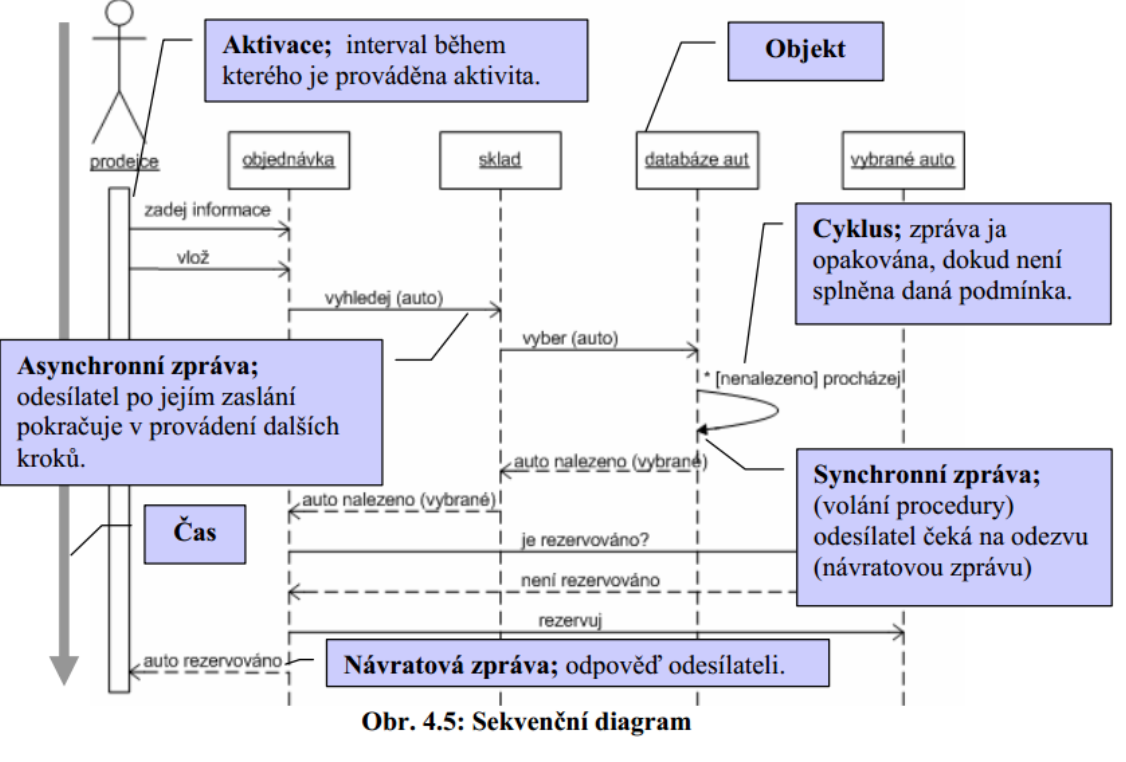
\includegraphics[width=1\textwidth]{assets/sekv}}

\pagebreak
\subsection{Diagram aktivit}
Diagram aktivit popisuje jednotlivé procesy pomocí aktivit reprezentující jeho (akční) \textbf{stavy} a \textbf{přechody mezi nimi}. Pokud aktivita "přetéká" v jednotlivých stavech mezi uživateli, mohou být tyto stavy naznačeny pomocí tzv \textbf{swimlines}.
\begin{figure}[H]
    \centering
    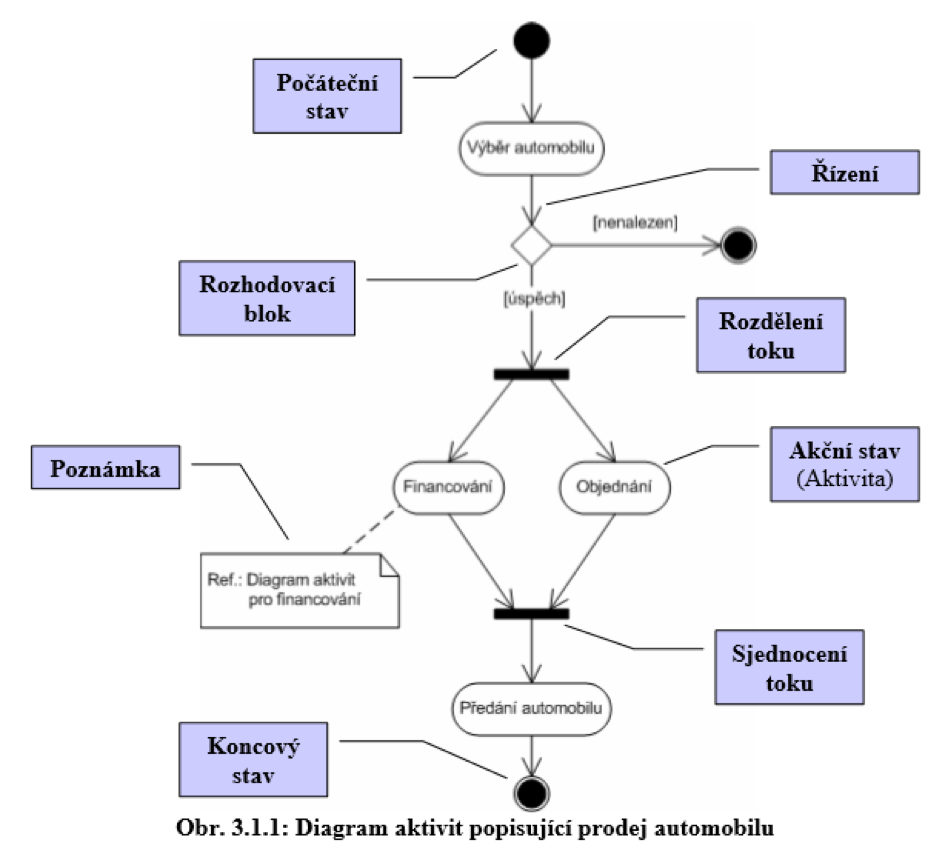
\includegraphics[width=1\textwidth]{assets/diag_aktivit.png}
\end{figure}

\begin{figure}[H]
	\centering
	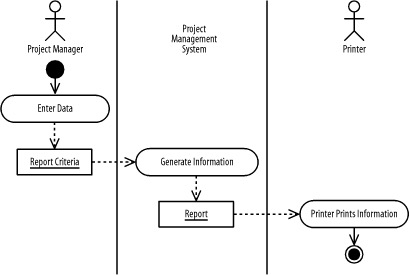
\includegraphics[width=1\textwidth]{assets/diag_aktivit_swimlines.gif}
\end{figure}
\pagebreak
\section{Křivky a plochy: teoretické základy (definice, rovnice, tečný a normálový vektor, křivosti, Cn a Gn spojitost), použití (Bézier, Coons, NURBS).}
Model návrhu dále \textbf{upřesňuje model analýzy ve světle skutečného implementačního prostředí}. Model návrhu tak představuje \textbf{druhou fázi} vývoje softwaru. Jde o abstrakci zdrojového kódu, která bude sloužit jako hlavní dokument programátorům v další implementační fázi.

\subsection{Návrh a jeho cíle}
Pojem implementační prostředí v podstatě vyjadřuje \textbf{možnost namapovat navržené softwarové komponenty} obsažené v modelu analýzy na architekturu systému určeného k provozu vyvíjené aplikace \textbf{s maximálním možným využitím služeb již existujících softwarových komponent}. Postup včlenění implementačního prostředí do vyvíjené aplikace je dán následující posloupností činností:
\begin{enumerate}
\item Definice \textbf{systémové architektury}.
\item Identifikace \textbf{návrhových vzorů} a možnosti znovupoužití tzv. rámcových řešení.
\item Definice softwarových komponent a jejich \textbf{znovupoužití}.
\end{enumerate}
V této fázi se uplatňují následující diagramy:

\begin{itemize}
\item \textbf{Diagram tříd} - specifikuje \textbf{množinu tříd, rozhraní a jejich vzájemné vztahy}. Tyto diagramy slouží k vyjádření \textbf{statického} pohledu na systém.
\item \textbf{Sekvenční diagram} - popisuje \textbf{interakce mezi objekty} z hlediska jejich \textbf{časového} uspořádaní.
\item \textbf{Diagram spolupráce} - je obdobně jako sekvenční diagram zaměřen na \textbf{interakce}, ale {z pohledu strukturální organizace objektů}. Jinými slovy není primárním aspektem časová posloupnost posílaných zpráv, ale \textbf{topologie rozmístění objektů}.
\item \textbf{Stavový diagram} - dokumentuje \textbf{životní cyklus objektu} dané třídy a stavy, ve kterých se může nacházet.
\item \textbf{Diagram nasazení} - popisuje \textbf{konfiguraci} (topologii) \textbf{technických prostředků} umožňující běh vlastního softwarového systému (rozmístění HW a SW).
\end{itemize}

\begin{figure}[H]
	\centering
	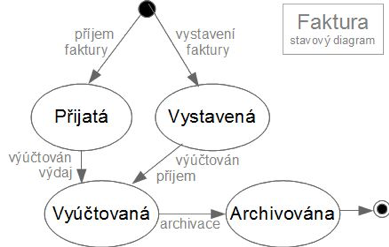
\includegraphics[width=.4\textwidth]{assets/diag_stavovy.png}
\end{figure}
\begin{figure}
	\centering
	\begin{minipage}{.5\textwidth}
		\centering
		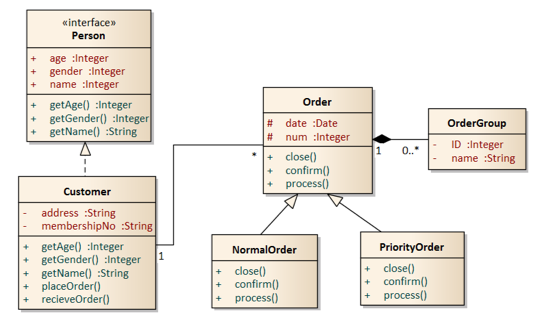
\includegraphics[width=.95\linewidth]{assets/diag_tridni.png}
	\end{minipage}%
	\begin{minipage}{.5\textwidth}
		\centering
		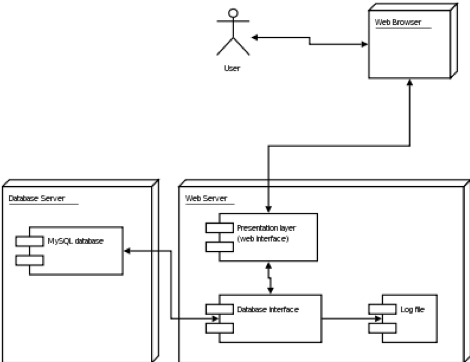
\includegraphics[width=.95\linewidth]{assets/diag_nasazeni.png}
	\end{minipage}
\end{figure}

\subsection{Návrhové vzory - členění}
Návrhové vzory jsou metodiky (šablony) pro \textbf{řešení různých problému}, se kterými se vývojář může setkat. Objektově orientované návrhové vzory typicky ukazují \textbf{vztahy} a \textbf{interakce mezi třídami a objekty}, aniž by určovaly implementaci konkrétní třídy. Dělí se do tří základních skupin:
\begin{itemize}
\item \textbf{Creational Patterns (vytvářející)} - určené k řešení problému vytváření instancí tříd cestou delegace této funkce na speciálně k tomuto účelu navržené třídy. Většinou se jedná o dynamická rozhodnutí učiněná za běhu programu.
\item \textbf{Structural Patterns (strukturální)} - představují skupinu návrhových vzorů zaměřujících se na možnosti uspořádání jednotlivých objektů a jejich tříd nebo komponent v systému. Snahou je zpřehlednit systém a využít možností strukturalizace kódu.
\item \textbf{Behavioral Patterns (chování)} - zajímají se o chování systému. Mohou být založeny na třídách nebo objektech. U tříd využívají při návrhu řešení především principu dědičnosti. V druhém přístupu je \textbf{řešena spolupráce mezi objekty a skupinami objektů}, která zajišťuje dosažení požadovaného výsledku.
\end{itemize}

\subsubsection{Creational patterns (Vzory týkající se tvorby objektů)}
\begin{itemize}
	\item \textbf{Abstract Factory (Abstraktní továrna)} - Definuje rozhraní pro vytváření rodin objektů, které jsou na sobě závislé nebo spolu nějak souvisí bez určení konkrétní třídy. Klient je odstíněn od vytváření konkrétních instancí objektů.
	\item \textbf{Factory Method (Tovární metoda)} - Definuje rozhraní pro vytváření objektu, které nechává potomky rozhodnout o tom, jaký objekt bude fakticky vytvořen. *Tovární metoda nechává třídy přenést vytváření na potomky.
	\item \textbf{Builder (Stavitel)} - Odděluje tvorbu komplexu objektů od jejich reprezentace tak, aby stejný proces tvorby mohl být použit i pro jiné reprezentace.
	\item \textbf{Singleton (Jedináček)} - Zajišťuje, že daná třída má pouze jednu instanci (využívá se privátních konstruktorů a samotná třída ve statické proměnné uchovává danou instanci).
	\item \textbf{Prototype (Prototyp, Klon)} - Specifikuje druh objektů, které se mají vytvořit použitím prototypového objektu. Nové objekty se vytváří kopírováním tohoto prototypového objektu.
\end{itemize}

\subsubsection{Structural Patterns (Vzory týkající se struktury programu)}
\begin{itemize}
	\item \textbf{Adapter (Adaptér)} - Potřebujete-li, aby spolu pracovaly dvě třídy, které nemají kompatibilní rozhraní. Adaptér převádí rozhraní jedné třídy na rozhraní druhé třídy.
	\item \textbf{Bridge (Most)} - Oddělí abstrakci od implementace, tak aby se tyto dvě mohly libovolně lišit.
	\item \textbf{Composite (Kompozit, Strom, Složenina)} - Komponuje objekty do stromové struktury a umožňuje klientovi pracovat s jednotlivými i se složenými objekty stejným způsobem.
	\item \textbf{Decorator (Dekorátor)} - Dekorátor se vytváří za účelem změny instancí tříd bez nutnosti vytvoření nových odvozených tříd, jelikož pouze dynamicky připojuje další funkčnosti k objektu. Nový objekt si zachovává původní rozhraní.
	\item \textbf{Facade (Fasáda)} - Nabízí jednotné rozhraní k sadě rozhraní v podsystému. Definuje rozhraní vyšší úrovně, které zjednodušuje použití podsystému.
	\item \textbf{Flyweight (Muší váha)} - Je vhodná pro použití v případě, že máte příliš mnoho malých objektů, které jsou si velmi podobné.
	\item \textbf{Proxy} - Nabízí náhradu nebo zástupný objekt za nějaký jiný pro kontrolu přístupu k danému objektu.
\end{itemize}

\subsubsection{Behavioral Patterns (Vzory týkající se chování)}
\begin{itemize}
	\item \textbf{Observer (Pozorovatel)} - V případě, kdy je na jednom objektu závislých mnoho dalších objektů, poskytne vám tento vzor způsob, jak všem dát vědět, když se něco změní. Observer je možné použít v situaci, kdy je definována závislost jednoho objektu na druhém. Závislost ve smyslu propagace změny nezávislého objektu závislým objektům (pozorovatelům). Nezávislý objekt musí informovat závislé objekty o \textbf{událostech}, které je mohou ovlivnit.
	\item \textbf{Command (Příkaz)} - Zapouzdřete požadavek jako objekt a tím umožněte parametrizovat klienty s různými požadavky, frontami nebo požadavky na log a podporujte operace, které jdou vzít zpět.
	\item \textbf{Interpreter (Interpret)} - Vytváří jazyk, což znamená definování gramatických pravidel a určení způsobu, jak vzniklý jazyk interpretovat.
	\item \textbf{State (Stav)} - Umožňuje objektu měnit své chování, pokud se změní jeho vnitřní stav. Objekt se tváří, jako kdyby se stal instancí jiné třídy.
	\item \textbf{Strategy (Strategie)} - Zapouzdřuje nějaký druh algoritmů nebo objektů, které se mají měnit, tak aby byly pro klienta zaměnitelné.
	\item \textbf{Chain of responsibility (Zřetězení zodpovědnosti)} - Řeší jak zaslat požadavek bez přesného vymezení objektu, který jej zpracuje.
	\item \textbf{Visitor (Návštěvník)} - Reprezentuje operaci, která by měla být provedena na elementech objektové struktury. Visitor vám umožní definovat nové operace beze změny tříd elementů na kterých pracuje.
	\item \textbf{Iterator (Iterátor)} - Řeší problém, jak se pohybovat mezi prvky, které jsou sekvenčně uspořádány, bez znalosti implementace jednotlivých prvků posloupnosti.
	\item \textbf{Mediator (Prostředník)} - Umožňuje zajistit komunikaci mezi dvěma komponentami programu, aniž by byly v přímé interakci a tím musely přesně znát poskytované metody.
	\item \textbf{Memento (Memento)} - Bez porušování zapouzdření zachyťte a uložte do externího objektu interní stav objektu tak, aby ten objekt mohl být do tohoto stavu kdykoliv později vrácen.
	\item \textbf{Template method (Šablonová metoda)} - Definuje kostru toho, jak nějaký algoritmus funguje, s tím, že některé kroky nechává na potomcích. Umožňuje tak potomkům upravit určité kroky algoritmu bez toho, aby mohli měnit strukturu algoritmu.
\end{itemize}

\pagebreak
\section{Geometrické a objemové modelování. Hraniční metoda, metoda CSG, výčet prostoru, oktantové stromy.}
\subsection{Procedurální rozšíření SQL}
Kromě základních příkazu pro vytváření a modifikací dat obsahuje PSQL triggery, funkce, procedury, kurzory. To umožňuje přenést část aplikační logiky přímo do databází. Je \textbf{závislé na SŘBD} a její různé implementace se mnohdy velice liší:
\begin{itemize}
\item \textbf{PL/SQL} pro Oracle
\item \textbf{Transact-SQL} (T-SQL) pro Sybase a MSSQL
\item \textbf{PL/pgSQL} pro PostgreSQL
\item \textbf{SQL PL} pro DB2
\end{itemize}

\subsection{PL/SQL}
\begin{itemize}
\item Založeno na jazyku ADA.
\item Kód uložen a \textbf{prováděn v SŘBD}, může být sdílen více aplikacemi.
\item \textbf{Nezávislý na aplikační platformě} (pouze na SŘBD).
\end{itemize}

\subsubsection{Proměnné, procedury a funkce}
\begin{itemize}
	\item \textbf{Proměnné}
\begin{itemize}
\item Proměnné můžeme rozdělit do několika skupin, dle různých kritérií, nejčastějším dělením je podle \textbf{datového typu} na \textbf{číselné} (NUMBER), \textbf{stringové} (CHAR, VARCHAR2), \textbf{datumové} (DATE, TIMESTAMP).
\item Definujeme proměnné \texttt{part\_no NUMBER(4); in\_stock BOOLEAN;}
\item Přiřazení do proměnných je pomocí operátoru \textbf{\texttt{:=}}.
\end{itemize}

\item \textbf{Anonymní procedury}
\begin{itemize}
\item \textbf{Nepojmenované} procedury které \textbf{nejde volat}.
\item Mohou být uloženy v souboru nebo spuštěny přímo z konzole.
\item Jsou pomalejší než pojmenované procedury, protože \textbf{nemohou být předkompilovány}.
\end{itemize}

\item \textbf{Pojmenované procedury}
\begin{itemize}
\item Obsahují \textbf{hlavičku se jménem a parametry}. Díky tomu se dají volat z jiných procedur či triggrů nebo spuštěny příkazem \textbf{EXECUTE}.
\item Jelikož jsou \textbf{kompilovány} jen jednou, jsou rychlejší než anonymní.
\item \texttt{CREATE [OR REPLACE] PROCEDURE jmeno\_procedury [( jmeno\_parametru [mod] datovy\_typ , ... )] IS|AS definice lokálních proměnných BEGIN tělo procedury END [jmeno\_procedury]}
\end{itemize}

\item \textbf{Funkce}
\begin{itemize}
\item Na rozdíl od procedury \textbf{vrací hodnotu}. Kromě standardních funkcí (\texttt{TO.CHAR, TO.DATE, SUBSTR}, apod.) si můžeme definovat \textbf{vlastní funkce}.
\item \texttt{CREATE [OR REPLACE] FUNCTION jmeno\_funkce [( jmeno\_parametru [mod] datovy\_typ , ... )] RETURN navratovy\_datovy\_typ IS |AS definice lokálních proměnných BEGIN tělo procedury END [jmeno\_procedury]}
\end{itemize}
\end{itemize}

\subsubsection{Dynamické a statické PL/SQL}
\begin{itemize}
\item \textbf{Statické PL/SQL} - klasické procedury, které mají vázané proměnné.
\item \textbf{Dynamické PL/SQL} - kód SQL příkazu je vytvářen dynamicky za běhu - vytvoření textového řetězce a jeho spuštění příkazem \textbf{\texttt{EXECUTE IMMEDIATE}}.
\end{itemize}

\subsubsection{Výjimky, podmínky, cykly}
\begin{itemize}
\item \textbf{Výjimky}
\begin{itemize}
\item Vznikají ručně i ze systému.
\item Zpracování v bloku \texttt{\textbf{EXCEPTION}}
\item Pro ruční vyvolání je nutné ji deklarovat (DECLARE vyjimka EXCEPTION;) a vyhodit (\textbf{\texttt{RAISE}} vyjimka)
\end{itemize}
\item \textbf{Podmínky}
\begin{itemize}
\item \texttt{IF podminka1 THEN příkazy [ELSIF podminka2 THEN příkazy ] [ELSE příkazy ] END IF ;}
\end{itemize}
\item \textbf{Cykly}
\begin{itemize}
\item \textbf{do while} - \texttt{LOOP příkazy cyklu [EXIT; | EXIT WHEN podminka ;] END LOOP;}
\item \textbf{while do} - \texttt{WHILE podminka LOOP příkazy cyklu END LOOP;}
\item \textbf{for} - \texttt{FOR jmeno\_promenne IN [REVERSE] value1 .. value2 LOOP příkazy cyklu END LOOP;}
\end{itemize}
\end{itemize}


\subsubsection{Kurzory, triggery, hromadné operace}
\begin{itemize}
\item\textbf{Triggery}
\begin{itemize}
\item Kód spouštěný v reakci na \textbf{událost} (DML, DDL, systémové eventy).
\item Pokud se pokusíme v triggeru číst či modifikovat stejnou tabulku dostaneme \textbf{mutating table error}.
\item \texttt{CREATE [OR REPLACE ] TRIGGER jmeno\_triggeru {BEFORE | AFTER | INSTEAD OF } {INSERT [OR] | UPDATE [OR] | DELETE} [OF jmeno\_sloupce] ON jmeno\_tabulky [REFERENCING OLD AS stara\_hodnota NEW AS nova\_hodnota] [FOR EACH ROW [WHEN (podminka )]] BEGIN příkazy END;}
\end{itemize}
\end{itemize}



\begin{itemize}
\item\textbf{Kurzory}
\begin{itemize}
\item Kurzor je ukazatel na řádek \textbf{víceřádkového výběru}. Je třeba jej v programu deklarovat pokud budeme zpracovávat víceřádkové výběry. Kurzorem mohu pohybovat a tak se dostanu na další řádky výběru. Jsou dva typy kurzoru:
\begin{itemize}
\item \textbf{implicitní} - vytváří se \textbf{automaticky} po provedení příkazu \texttt{INSERT}, \texttt{UPDATE}, \texttt{DELETE}.
\item \textbf{explicitní} - \textbf{ručně vytvořený kurzor}. Vytváří se nejčastěji ve spojením s příkazem \texttt{SELECT}.
\end{itemize}
\item \textbf{Příkazy pro práci s kurzorem:}
\begin{itemize}
\item \texttt{CURSOR kurzor IS select;} - vytvoření kurzoru.
\item \texttt{OPEN kurzor} - otevře kurzor, tedy nastaví ho na první řádek.
\item \texttt{FETCH kurzor INTO promena} - příkaz pro pohyb kurzoru. Načte aktuální záznam do proměnné a posune se na další záznam.
\item \texttt{CLOSE kurzor} - uzavře kurzor.
\end{itemize}
\end{itemize}


\item\textbf{Vázané proměnné}
\begin{itemize}
\item SŘBD kontroluje \textbf{jedinečnost dotazu}, pokud už byl dotaz v minulosti proveden, použije se \textbf{dříve použitý plán} dotazu místo nového vytváření plánu.
\item Vázané proměnné umožňují \textbf{parametrizaci hodnot v dotazu}, odpadá tedy opětovné vytváření plánu pro stejný dotaz s jinou hodnotou.
\item Lze používat i v dynamickém PL/SQL (pomocí \textbf{USING}).
\item Použití i při voláni z aplikace (podpora v C\# i Java).
\end{itemize}



\item\textbf{Hromadné operace}
\begin{itemize}
\item Snížení režie na zotavení (zápis do logu) a aktualizace DB (datových struktur). Výsledkem je rychlejší vkládání záznamů do DB.
\item Lze použít pro statické i dynamické SQL.
\item \textbf{\texttt{BULK COLLECT}}
\begin{itemize}
\item \textbf{Hromadné načtení} (navázání vstupní kolekce s PL/SQL enginem).
\item \texttt{BULK COLLECT INTO collection\_name[, collection\_name]}
\end{itemize}

\item \textbf{\texttt{FORALL}}
\begin{itemize}
\item Hromadná \textbf{operace} (navázání vstupní kolekce před posláním do SQL enginu)
\item \texttt{FORALL index IN lower\_bound..upper\_bound [INSERT, UPDATE nebo DELETE];}
\end{itemize}
\end{itemize}



\item\textbf{Balíky}
\begin{itemize}
\item Obdoba kníhoven v programovacích jazycích.
\item Specifikace balíku a následně tělo. 
\end{itemize}


\end{itemize}






\subsection{T-SQL (Transact-SQL)}
Transact-SQL (T-SQL) je proprietární rozšíření jazyka SQL od společností \textbf{Microsoft} a \textbf{Sybase}, které Microsoft používá v produktu \textbf{Microsoft SQL Server}, Sybase Software pak v Adaptive Server Enterprise.

\subsubsection{Proměnné, procedury a funkce}
\begin{itemize}
\item \textbf{Proměnné}
\begin{itemize}
\item \textbf{Deklarace} pomocí \texttt{DECLARE @TMP INT}.
\item \textbf{Inicializace} pomocí \texttt{SET} nebo \texttt{SELECT}.
\end{itemize}

\item \textbf{Podmínky}
\begin{itemize}
\item \texttt{IF <boolean condition > <statement> ELSE <statement>}
\item Více příkazů v jedné větvi musíme obalit do \texttt{BEGIN/END}.
\end{itemize}


\item \textbf{Cykly}
\begin{itemize}
\item \texttt{WHILE <Boolean expression> <code block>}
\end{itemize}


\item \textbf{Transakce}
\begin{itemize}
\item \textbf{Začátek} - \texttt{BEGIN TRANSACTION <nazev\_transakce>}
\item \textbf{Konec} - \texttt{ROLLBACK nebo COMMIT}
\item \textbf{Nastavení úrovně izolace} - \texttt{SET TRANSACTION ISOLATION LEVEL <level>}
\end{itemize}


\item \textbf{Výjimky}
\begin{itemize}
\item Bloky try/catch (BEGIN TRY/END TRY a BEGIN CATCH/END CATCH).
\end{itemize}


\item \textbf{Uložené procedury}
\begin{itemize}
\item Uloženy v SŘBD.
\item Předkompilovány, tudíž jsou rychlejší.
\item \texttt{CREATE PROC[EDURE] procedure\_name [;number] [{ @parameter data\_type } [VARYING] [= default ] [OUTPUT] ] [ , . . . ] [ WITH { RECOMPILE | ENCRYPTION | RECOMPILE, ENCRYPTION } ] [FOR REPLICATION] AS sql\_statement}
\end{itemize}


\item \textbf{Uložené funkce}
\begin{itemize}
\item Není možné použít try/catch, DML atd.
\item Musí vracet hodnotu.
\item \texttt{CREATE FUNCTION [ schema\_name. ] function\_name ( [ { @parameter\_name [ AS ][ type\_schema\_name .] parameter\_data\_type [ = default ] [ READONLY ] } [ ,...n ] ] ) RETURNS return\_data\_type [ WITH <function\_option > [ ,...n ] ] [ AS ] BEGIN function\_body RETURN scalar\_expression END [ ; ]}
\end{itemize}
\end{itemize}



\subsubsection{Kurzory, triggery, dynamické SQL}
\begin{itemize}
\item \textbf{Kurzory}
\begin{itemize}
\item \texttt{DECLARE cursor\_name CURSOR FOR select\_statement }
\item \textbf{Musíme použít} sekvenci příkazů: \texttt{OPEN, FETCH, CLOSE, DEALLOCATE }
\item Pro testování prázdného kurzoru používáme \texttt{@@FETCH\_STATUS}
\end{itemize}

\item \textbf{Trigger}
\begin{itemize}
\item \texttt{CREATE TRIGGER [ schema\_name . ] trigger\_name ON { table | view } [ WITH <dml\_trigger\_option > [ ,...n ] ] { FOR | AFTER | INSTEAD OF } { [ INSERT ] [ , ] [ UPDATE ] [ , ] [ DELETE ] } [ WITH APPEND ] [ NOT FOR REPLICATION ] AS { sql\_statement [ ; ] [ ,...n ] | EXTERNAL NAME <method specifier [ ; ] > }}
\end{itemize}

\item \textbf{Dynamické SQL}
\begin{itemize}
\item Podobné PL/SQL, pomocí příkazu \textbf{\texttt{sp\_executesql}}
\item \texttt{sp\_executesql [@stmt =] stmt [ { , [@params =] N’@parameter\_name data\_type [ ,... n] ’ } { , [@param1 =] ’value1 ’ [ ,... n] } ]}
\end{itemize}
\end{itemize}



\subsection{Rozdíly PL/SQL vs T-SQL}
\begin{itemize}
\item \textbf{T-SQL} \textbf{neposkytuje operátory} jako \texttt{\%TYPE} a \texttt{\%ROWTYPE} pro získání datových typů existujících záznamů.
\item \textbf{T-SQL} \textbf{nepodporuje} \texttt{CREATE OR REPLACE PROCEDURE}, což nás nutí k tomuto zápisu: \texttt{/*CREATE*/ ALTER PROCEDURE}.
\item \textbf{T-SQL} podstatně \textbf{omezuje konstrukce}, které můžeme využívat ve funkcích.
\item V \textbf{T-SQL} musím při práci s kurzory používat \texttt{OPEN}, \texttt{FETCH}, \texttt{CLOSE}, \texttt{DEALLOCATE}.
\item \textbf{T-SQL} nás nutí k dvojitému \texttt{FETCH} u kurzorů. 
\item V \textbf{T-SQL} musíme definovat u parametrů procedur a funkcí \textbf{délku datového typu} (pokud se u datového typu udává).
\item V \textbf{T-SQL} musíme více příkazů v jedné větvi obalit do \texttt{BEGIN/END}.
\end{itemize}



\pagebreak
\section{Standardní zobrazovací řetězec a realizace jeho jednotlivých kroků. Gouraudovo a Phongovo stínování. Řešení viditelnosti. Grafický standard OpenGL: stručná charakteristika.}
\subsection{Fyzicka implementace}
Fyzická implementace definuje \textbf{datové struktury} pro základní logické objekty:

\begin{itemize}
\item \textbf{tabulky},
\item \textbf{indexy},
\item \textbf{materializované pohledy} (materialized views),
\item \textbf{rozdělení dat} (data partitioning) --  data s dlouhou historií. Fyzické rozdělení datových struktur a souboru na více částí.
\end{itemize}

Fyzická implementace tedy \textbf{řeší uložení dat na nejnižší úrovni databáze}.
 Na úrovni databáze můžeme ovlivnit výběr efektivnějšího plánu vykonávání dotazu případně \textbf{dobu vykonávání operací}.

\begin{itemize}
\item \textbf{ROWID} -- jedinečné číslo \textbf{označující záznam tabulky}.
\item Větší část teorie fyzického návrhu DB je platná pro libovolné SŘBD, dále se musíme řídit \textbf{doporučením výrobce}.
\item Každé SŘBD obsahuje specifickou reprezentaci tabulek a indexů:
\begin{itemize}
\item \textbf{CREATE TABLE} - vytvoření tabulky typu \textbf{halda} (Oracle), \textbf{shlukování záznamů} (SQL Server 2012).
\item \textbf{CREATE INDEX} - vytvoření\textbf{ B+-stromu}, kde každá položka odkazuje na ROWID záznamu v tabulce.
\end{itemize}
\end{itemize}

\subsection{Datové struktury}
Datové struktury \textbf{se skládají} buďto ze \textbf{stránek}, nebo z \textbf{uzlů} v případě stromové struktury. Jsou realizovány tak aby \textbf{operace} vyhledávání, vkládání, editace a mazání \textbf{byly co nejefektivnější}. 

Pro rychlé vyhledávání, které předchází i editaci a mazání je \textbf{nutné udržovat datovou strukturu setříděnou}. To však může zpomalit operaci vkládání (např. zařazením nového záznamu doprostřed tabulky musím posunout milion záznamů).
Základní datové struktury:

\begin{itemize}
\item \textbf{Blok} (alokační jednotka) -- je nejmenší jednotka, se kterou SŘBD manipuluje při zápisu a čtení dat z disku (obvykle 4KB nebo 8KB).
\item \textbf{Stránka} -- nejmenší jednotka s kterou pracuje správce paměti. \texttt{Stranka.velikost = X * Blok.velikost} (je-li velikost bloku = 4KB je odpovídá velikost stránky násobkům 4KB).
\item \textbf{Datový soubor} -- fyzický prostor na disku s daty.
\end{itemize}


\subsection{Typy tabulek}
\subsubsection{Heap Table}
\begin{itemize}
\item Implicitní pro \texttt{CREATE TABLE} (v MSSQL), záznamy nejsou nijak uspořádány.
\item \textbf{Stránkové perzistentní pole} s velikostí \textbf{bloku} nejčastěji \textbf{8kB}.
\item Záznamy pouze \textbf{označovány jako smazané}, pro fyzické smazání slouží speciální operace \textbf{shrinking}.
\item Při vkládání záznam uložen na \textbf{první volnou pozici v tabulce} nebo na \textbf{konec pole}.
\item Složitost operací: neefektivní vyhledávání $O(n)$, velmi \textbf{efektivní vkládání} $O(1)$ i \textbf{využití místa}.
\end{itemize}
\subsubsection{Shlukování záznamů (Data Clustering)}
\begin{itemize}
\item Záznamy v \textbf{datovém souboru jsou seřazeny podle zvoleného klíče}, pro implementaci nejčastěji využita nějaká \textbf{varianta B-stromu}.
\item Listové uzly stromu (bloky) obsahují \textbf{kromě klíče i další záznamy} tabulky.
\item Používá se všude, kde potřebujeme \textbf{získat i hodnoty ostatních atributů} (kromě klíče - např. \texttt{SELECT} neklíčových atributů).
\item \textbf{Zhoršený výkon} \texttt{INSERT} (data se musí zatřizovat).
\item \textbf{Oracle:} Index Organized Table (IOT), \textbf{SQL Server:} Clustered Index.
\end{itemize}

\subsubsection{Hašovaná tabulka (Hash Table)}
\begin{itemize}
\item Záznamy se stejnou hashovanou hodnou jsou uloženy ve stejném nebo velmi blízkém bloku.
\item Trochu \textbf{plýtvá místem}.
\item Musíme znát předem velikost záznamů (alespoň přibližně).
\end{itemize}

\subsubsection{Materializované pohled (Materialized views)}
\begin{itemize}
\item Uložené \textbf{výsledky dotazů}, které bývají často v DB vyhodnocovány.
\item Jde spíše o \textbf{fragment} z \textbf{tabulky} či několika tabulek.
\end{itemize}

\subsection{Indexy}
Indexové soubory slouží k \textbf{seřazení tabulky podle jiných atributů než je samotná tabulka defaultně seřazená}. Index je tedy vázaný ke konkrétní tabulce a konkrétnímu atributu podle kterého data řadí. Index umožňuje \textbf{rychlé vyhledávání} dle klíče, \textbf{ROWID pak odkazuje na kompletní záznam v heap tabulce}. \texttt{CREATE [BITMAP] INDEX login ON Student;}. 
\begin{itemize}
\item \textbf{Primární index (PRIMARY)} -- automatický index, který se váže k primárnímu klíči, zajišťuje jedinečnost údajů.
\item \textbf{Unikátní index (UNIQUE)} -- stejně jako primární index zajišťuje jedinečnost údajů v atributu, ale neváže se pouze ke klíči.
\item \textbf{Vedlejší index (INDEX)} -- klasické index popsány níže.
\item \textbf{Fulltextový index} -- používá se pro optimalizaci fulltextového vyhledávání v daném sloupci.
\end{itemize}

\subsubsection{Bitmapový index}
\textbf{Odpovídá na všechny možné hodnoty daného atributu}. Jde o tabulku jedniček a nul, kde řádky reprezentují záznamy v indexované tabulce a sloupce hodnoty indexovaného atributu. Jednička pak znamená true, že záznam má hodnotu danou sloupcem. \textbf{Vyplatí se}, pokud se používají logické operátory (\texttt{AND}, \texttt{OR}, \texttt{XOR}) \textbf{nad několika bitmapovými indexy atributů}.

\begin{figure}[H]
	\centering
	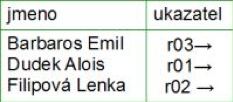
\includegraphics[width=0.3\textwidth]{assets/index_classic.png}
	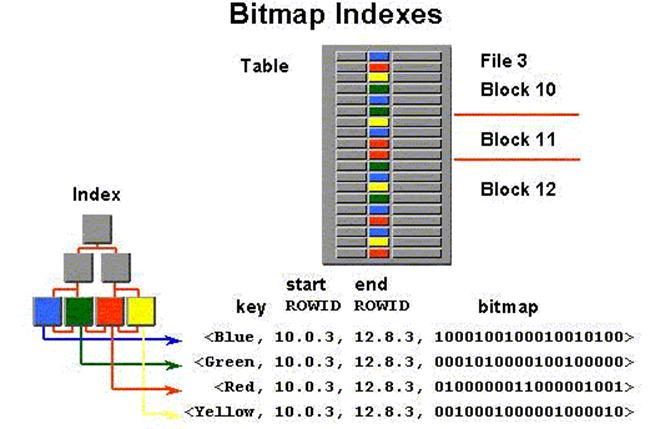
\includegraphics[width=0.65\textwidth]{assets/index_bitmap.jpg}
\end{figure}

\subsubsection{Shlukovaný index (Cluster Index)}
Pokud se pro dvě tabulky často používá operace spojeni (JOIN) pro jeden atribut. V tomto případě diskový blok obsahuje záznam z řídicí tabulky a zároveň i závislé záznamy. (v normalnim připadě obsahuje diskovy blok pouze zaznamy jedne tabulky).

\subsubsection{Kandidáti na index}
\begin{itemize}
\item \textbf{Primární} klíče a \textbf{cizí} klíče.
\item Pokud je index používán pro nalezení malého počtu záznamů.
\item Pokud index pokryje jeden nebo více častých dotazů.
\item Atributy často se vyskytující v konstrukci \texttt{WHERE}.
\end{itemize}

\subsection{Vykonávání dotazu}
\textbf{Ovlivnění času vykonávání dotazu} - parametrizované dotazy, hromadné operace, nastavení transakcí. Na úrovni DB můžeme ovlivnit výběr efektivnějšího plánu vykonávání dotazu, případně dobu vykonávání operací -> \textbf{fyzický návrh DB}. Identifikujeme \textbf{4 fáze vykonávání dotazu}:

\begin{enumerate}
	\item \textbf{Převod dotazu do interní formy}
	\begin{itemize}
		\item Převod původního dotazu do zvolené \textbf{interní formy}.
		\item \textbf{Eliminujeme syntaxi jazyka dotazu} (např. SQL).
		\item Zpracování pohledů, které probíhá v této fázi, znamená, že \textbf{nahradíme pohled jeho definicí} (materializované pohledy -- fragmenty/výsledky dotazů).
		\item Interní forma je nejčastěji \textbf{nějaký druh dotazovacího strom}u (angl. query tree).
	\end{itemize}
	\item \textbf{Převod do kanonické formy}
	\begin{itemize}
		\item V této fázi optimalizátor provádí celou řadu \textbf{optimalizací}.
		\item Převodem do kanonické formy dochází k \textbf{odstranění} různých povrchních \textbf{rozdílů} a především nalezení \textbf{efektivnějšího} \textbf{tvaru} než nabízel původní dotaz.
		\item \textbf{Optimalizátor} – transformační pravidla (převádí výraz na ekvivalentní). Fáze transformace/přepsání dotazu (query rewite). Dotaz tedy není ve skutečnosti vykonán přesně tak, jak byl zadán! 
	\end{itemize}
	\item \textbf{Výběr nízkoúrovňových procedur}
	\begin{itemize}
		\item V této fázi se optimalizátor rozhoduje jak bude transformovaný dotaz vykonán.
		\item Nyní optimalizátor uvažuje: \textbf{existenci indexů}, \textbf{distribuci hodnot}, \textbf{shlukování uložených dat}.
	\end{itemize}
	\item \textbf{Vygenerování plánů dotazu a výběr nejlevnějšího plánu}
	\begin{itemize}
		\item Cena procedury je závislá na aktuální \textbf{mohutnosti vstupních relací} a na mohutnosti \textbf{mezivýsledků jednotlivých procedur}.
		\item Odhad velikosti mezivýsledků je však často problematický jelikož velmi ovlivňuje cenu operace, jedná se o jeden z \textbf{nejřešenějších problémů}.
		\item Z množiny dotazovacích plánů pak \textbf{optimalizátor} vybírá ten \textbf{nejlepší}, tedy \textbf{nejlevnější}.
	\end{itemize}
\end{enumerate}

\subsection{Ladění dotazů}
\begin{itemize}
	\item Po vybrání nejlevnějšího plánu je \textbf{dotaz proveden} a uživateli vrácen výsledek.
	\item \textbf{Plán} lze v SŘBD většinou \textbf{zobrazit} - operace jako průchod tabulkou, přístup k indexu, třídění spojení atd. To lze využít pro \textbf{odladění dotazu} - např. uvidíme, že musíme použít index na neindexovaný atribut.
	\item Dvěma či více \textbf{různými dotazy} je možno obdržet \textbf{stejná data}. 
	\item \textbf{Rychlost} různých dotazů ovšem\textbf{ nemusí být stejná }i přesto, že vracejí stejná data.
	\item Snažíme dosáhnout \textbf{maximálního} \textbf{výkonu} se \textbf{stávajícími prostředky}.
	\item Plán vykonávání dotazu vybírá \textbf{optimalizátor}.
	\item Snažíme se vytvořit dotaz, který\textbf{ bude načítat z úložiště pouze to, co potřebuje}.
\end{itemize}

\subsubsection{Přístupy k ladění}
\begin{itemize}
\item \textbf{Proaktivní} -- Analyzujeme fyzický návrh a provádíme změny k lepšímu fungování.
\item \textbf{Reaktivní} -- Reagujeme na problém.
\end{itemize}

\subsubsection{Ladění výkonu SŘBD}
\begin{itemize}
	\item \textbf{HW} -- RAID, RAM, CPU (Poslení možnost, je to drahé, efektivnější je \textbf{vyladit fyzický návrh}).
	\item \textbf{Parametry SŘBD} -- Velikosti \textbf{cache}, maximum zámků, atd. Nutné optimalizovat na určité použití.
	\item \textbf{ORM} -- Minimum SQL příkazů a objemu přenášených dat. Úroveň izolace transakce.
\end{itemize}
\pagebreak
\section{Metody získávání fotorealistických obrázků (rekurzivní sledování paprsku, vyzařovací metoda, renderovací rovnice).}
\subsection{Správa paměti}
Správa paměti je v soubor metod, které operační systém používá při \textbf{přidělování operační paměti jednotlivým spuštěným procesům}.

\subsubsection*{Výhody Automatické správy paměti}
\begin{itemize}
\item Programátor se může věnovat řešení skutečného problému.
\item Rozhraní modulů jsou přehlednější -- není třeba řešit problém zodpovědnosti za uvolnění paměti pro objekty vytvořené různými moduly.
\item Nastává \textbf{menší množství chyb} spojených s přístupem do paměti.
\item Správa paměti je často pro nezkušené uživatele mnohem \textbf{efektivnější}.
\end{itemize}

\subsubsection*{Nevýhody Automatické správy paměti}
\begin{itemize}
\item Paměť může být zachována jen proto, že je dostupná, i když není dále využita.
\item Automatická správa paměti není k dispozici ve starších, ale často používaných jazycích.
\item Může navíc využívat další zdroje PC a mít tak dopad na výkon (GC).
\end{itemize}

\subsection{Úrovně správy paměti}
\begin{itemize}
	\item \textbf{Technické vybavení} -- registry, cache
	\item \textbf{Operační systém} -- virtuální paměť, segmentace, stránkování
	\item \textbf{Aplikace} -- přidělování paměti, regenerace paměti:
	\begin{itemize}
		\item \textbf{Manuální} -- delete, dispose, free()
		\item \textbf{Automatická} -- garbage collector
	\end{itemize}
\end{itemize}

\subsection{Správa paměti v jednotlivých jazycích}
Pro zjištění toho, které úseky paměti se již nepoužívají, je k dispozici mnoho algoritmů. Většinou spoléhá automatická regenerace paměti na informace o tom, na které bloky paměti \textbf{neukazuje žádná programová proměnná}. V zásadě existují \textbf{dvě} \textbf{skupiny} metod:
\begin{itemize}
	\item metody založené na \textbf{sledování odkazů},
	\item metody založené na \textbf{čítačích odkazů}.
\end{itemize}

\subsubsection{C}
Jazyk C umožňuje spravovat paměť staticky (automaticky) a dynamicky. \textbf{Staticky} alokované proměnné jsou umístěny do hlavní paměti (velice často s výkoným kódem programu). \textbf{Automaticky} alokované proměnné se alokují na zásobníků a vznikají/zanikají podle potřeb programu. Pro tyto proměnné platí, že jejich velikost musí být známá v čase kompilace.

\textbf{Dynamická} správa paměti je plně v \textbf{rukou programátora} a využívá se \textbf{4 funkcí} (\texttt{malloc}, \texttt{realloc}, \texttt{calloc}, \texttt{free}). Typicky je paměť alokována na haldě a přistupuje se k ní pomocí ukazatelů. 

\subsubsection{C++}
C++ poskytuje mnoho způsobů jak na správu paměti, od \textbf{automatické} po \textbf{manuální} pomocí operátorů \texttt{new} a \texttt{delete}. \textbf{Automatická správa paměti} alokovaných objektů je z velké části postavena na návrhovém vzoru \textbf{RAII} (Resource Aquisition Is Initialization) -- správa zdrojů daného objektu je vázána na jeho životnost a jeho destruktor je povinen jejich uvolnění. Jednoduše stačí získat zdroj (paměť, soubor, grafický handle, cokoli) a uložit ho do proměnné, která ho bude vlastnit a při jejím zániku (voláním destruktoru) ho také uvolní. A tím se o to můžete přestat starat, protože zbytek zařídí C++ kompilátor, který bude uvolňovat zdroje automaticky v rámci rušení lokálních proměnných na konci oboru platnosti (scope). Mezi \textbf{výhody} RAII patří:
\begin{itemize}
\item RAII uklízí nejenom paměť, ale všechny zdroje (soubory, mutex, databáze, transakce, síťové sockety).
\item Úklid je proveden okamžitě bez prodlení, přesně v čase kdy zdroj přestává být potřeba.
\item Proměnné a zdroje likviduje po skončení platnosti stejný thread, který je vytvořil.
\item Není třeba zastavovat program kvůli GC jako v případě Javy, LISPu, atd.
\end{itemize}
Má však i \textbf{nevýhody}:
\begin{itemize}
\item Je nepatrně pomalejší, protože dealokuje okamžitě jeden podruhém, zatímco klasické GC dealokují naráz větší množství paměti.
\item Je třeba podpoře RAII věnovat pozornost při implementaci tříd (implementace destruktoru).
\end{itemize}

\textbf{Smart pointry} představují další způsob jak na automatickou správu paměti dynamicky alokovaných objektů. SP jsou definované jako třída, která overloaduje operátory \texttt{->}, \texttt{*}, \texttt{->*}, což ji umožňuje ,,chovat se jako pointer'' a fungovat ve většině kódu v kombinaci s reálnými a smart pointry. Existuje mnoho typů, které definují typ vlastnictví a podmínky, za nichž je objekt dealokován (\texttt{shared\_ptr}, \texttt{weak\_ptr}, \texttt{unique\_ptr}). Princip dealokace je stejný jako u RAII.

\subsubsection{C\#}
Správa paměti je v jazyce C\# \textbf{plně automatizovaná}, paměťový prostor se přiděluje operátorem \textbf{new} a jeho uvolnění zajistí systém \textbf{řízení běhu programu}. V \textbf{.NET} se používá varianta GC v podobě \textbf{Mark \& Sweep}.

V případě, že pracujeme s \textbf{neřízenými zdroji} (systémové zdroje -- soubory, připojení k DB, síť), které je třeba \textbf{explicitně uvolnit}, implementuje se rozhraní \textbf{IDisposable}. To předepisuje jedinou metodu \texttt{Dispose()}, kterou je třeba zavolat po skončení práce s objektem (stará se o uvolnění zdrojů, samotný objekt poté existuje dál až do uvolnění GC).

Dále lze v .NET definovat u tříd i tzv. safe-guard v podobě \textbf{finalizer} (metoda, která se volá při uklízení objektu pomocí GC). Syntaxe je podobná C++ (\texttt{\textasciitilde{}ClassName()}). Jelikož však zhoršuje efektivitu, definuje se pouze u tříd s rozhraním IDisposable. Jeho cílem je uvolnit zdroje, \textbf{pokud uživatel objektu nezavolá/zapomene zavolat} metodu \texttt{Dispose()}. 

\subsubsection{Java}
V jazyce Java je správa paměti rovněž \textbf{plně automatizovaná} a o její uvolnění se stará GC (varianta Mark \& Sweep). Java uchovává všechny reference na Stacku a na heapu vytváří objekty. Programátor má možnost vytvářet \textbf{strong} (klasická), \textbf{weak} (pokud na objekt ukazují pouze weak reference, tak bude uvolněn), \textbf{soft} (zajištěno uvolnění při nedostatku paměti před vyhozením chyby \texttt{outOfMemory}) reference, které definují kdy bude objekt dealokován.

Speciálním případem jsou Stringy (jsou \textbf{immutable}), kdy Java spravuje tzv. \textbf{String pool}. To znamená, že si ukládá a snaží se stringy znovupoužívat jak je to možné. To neplatí pro stringy, které jsou vypočítány, pouze pro konstanty. Můžeme však přinutit JVM k vložení těchto stringů do poolu pomocí metody \texttt{.intern()}. V Javě existují \textbf{3 typy GC}:
\begin{itemize}
\item \textbf{Serial GC} -- kolektor, který běží pouze v jednom jádře (malé aplikace, malé využití dat).
\item \textbf{Parallel GC} -- oproti serial využívá více threadů.
\item \textbf{Mostly concurent GC} -- při běhu GC vždy dojde k pozastavení aplikace, tento GC se tomu snaží předejít tak, že jede \textbf{souběžně} s aplikací. Nefunguje však souběžně 100\% času, kdy je někdy nutné program pozastavit, tyto pauzy se však snaží být co nejkratší pro zajištění co nejlepšího výkonu.
\end{itemize}

Podobně jako v C\#, Java poskytuje rozhraní \texttt{AutoCloseable}, které poskytuje operaci \texttt{close()}. Nejedná se o přímého zástupce za IDisposable, ale toto rozhranní umožňuje v javě využívat tzv. \textbf{try-with-resources} (ekvivalent v C\# using), kdy dochází k automatickému zavolání metody \texttt{close()} na konci \texttt{try-catch} bloku v části \texttt{finally}.

\subsection{Garbage collector (GC)}
Je obvykle část běhového prostředí (programovacího) jazyka, nebo přídavná knihovna (podporovaná kompilátorem, hardware, operačním systémem, nebo jakoukoli kombinací těchto tří). Má za úkol \textbf{automaticky} \textbf{určit}, která část \textbf{paměti} programu je už \textbf{nepoužívaná}, a připravit ji pro další znovupoužití.

\subsubsection{Mark \& Sweep}
Algoritmus nejdříve nastaví všem objektům, které jsou v paměti, \textbf{speciální příznak} navštíven na hodnotu ne. Poté projde všechny objekty, ke kterým se lze dostat. Těm, které takto navštívil, nastaví příznak na hodnotu ano. V okamžiku, kdy se už nemůže dostat k žádnému dalšímu objektu, znamená to, že všechny objekty s příznakem navštíven majícím hodnotu ne jsou odpad -- a mohou být tedy uvolněny z paměti.

Tato metoda má několik nevýhod. Největší je, že při garbage collectionu je \textbf{přerušen běh programu}. To znamená,že programy \textbf{pravidelně zamrznou}, takže je nemožné pracovat s aplikacemi pracujícími v reálném čase.

\subsubsection{Reference counting}
Ke každému objektu je přiřazen \textbf{čítač referencí}. Když je objekt vytvořen, jeho čítači je nastaven na \textbf{hodnotu 1}. V okamžiku, kdy si nějaký jiný objekt uloží referenci na tento objekt, hodnota čítače je \textbf{zvětšena o 1}. Ve chvíli, kdy je reference mimo rozsah platnosti (např. po opuštění funkce, která si referenci uložila), nebo když je referenci přiřazena nová hodnota, čítač je \textbf{snížen o 1}. Jestliže je hodnota čítače některého objektu nulová, může být tento objekt uvolněn z paměti.

\subsubsection{Generační algoritmus}
Staví na \textbf{dvou základních principech}:
\begin{itemize}
\item Mnoho objektů se stane \textbf{odpadem} krátce \textbf{po} svém \textbf{vzniku}.
\item Jen malé procento \textbf{referencí} ve „starších“ objektech \textbf{ukazuje na objekty mladší}.
\end{itemize}
\textbf{Rozděluje si paměť programu do několika částí}, tzv. „\textbf{generací}“. Objekty jsou vytvářeny ve spodní (nejmladší) generaci a po splnění určité podmínky, obvykle stáří), jsou přeřazeny do starší generace. Pro každou generaci může být \textbf{úklid} prováděn v rozdílných \textbf{časových intervalech }(nejkratší intervaly obvykle budou platit pro nejmladší generaci) a dokonce pro rozdílné generace mohou být použity \textbf{rozdílné algoritmy úklidu}. V okamžiku, kdy se prostor pro spodní generaci zaplní, všechny dosažitelné objekty v nejmladší generaci jsou zkopírovány do starší generace. I tak bude množství kopírovaných objektů pouze zlomkem z celkového množství mladších objektů, jelikož většina z nich se již stala odpadem.

\subsubsection{Nevýhody GC}
\begin{itemize}
\item Garbage collector potřebuje ke své práci \textbf{procesorový čas}, aby mohl rozhodovat o tom, jestli je objekt v paměti „mrtvý“, nebo „živý“.
\item Některé garbage collectory mohou způsobit i dosti znatelné \textbf{pauzy}, což je vážný problém pro systémy běžící v reálném čase.
\item O stavu objektů musí mít garbage collector uloženou informaci. Tyto informace vyžadují určitou \textbf{paměť navíc}.
\item Některé jazyky s garbage collectorem neumožňují programátorovi \textbf{znovupoužití paměti}, i když ví, že paměť už nebude použita. To vede k \textbf{nárůstu alokace paměti}.
\end{itemize}

\subsection{Virtuální stroj}
Je v informatice software, který vytváří \textbf{virtualizované prostředí} mezi platformou počítače (HW i SW) a operačním systémem, ve kterém koncový uživatel může provozovat software na \textbf{abstraktním stroji}.

\subsubsection{Hardwarový virtuální stroj}
Původní význam pro virtuální stroj, někdy nazývaný též hardwarový virtuální stroj, označuje \textbf{několik jednotlivých totožných pracovních prostředí na jediném počítači}, z nichž na každém běží operační systém. Díky tomu může být aplikace psaná pro jeden OS používána na stroji, na kterém běží jiný OS, nebo zajišťuje vykonání sandboxu, který poskytuje větší úroveň izolace mezi procesy, než je dosaženo při vykonávání několika procesů najednou (multitasking) na stejném OS.

Jedním využitím může být také poskytnutí iluze mnoha uživatelům, že používají celý počítač, který je jejich „soukromým“ strojem, izolovaným od ostatních uživatelů, přestože všichni používají jeden fyzický stroj. Další výhodou může být to, že start (bootování) a restart virtuálního počítače může být mnohem rychlejší, než u fyzického stroje, protože mohou být přeskočeny úkoly jako například inicializace hardwaru.

Podobný software je často označován termíny jako virtualizace a virtuální servery. Hostitelský software, který poskytuje tuto schopnost je často označovaný jako \textbf{hypervisor} nebovirtuální strojový monitor (virtual machine monitor).
\textbf{Softwarové virtualizace} mohou být prováděny \textbf{ve třech hlavních úrovních}:
\begin{itemize}
\item \textbf{Emulace} -- virtuální stroj simuluje kompletní hardware, dovolující provoz nemodifikovaného OS na úplně jiném procesoru.
\item\textbf{Paravirtualizace} -- virtuální stroj nesimuluje hardware, ale místo toho nabídne \textbf{speciální rozhraní API}, které vyžaduje určité modifikace hostovaného operačního systému, aby mohl být tento OS nad virtuálním strojem spouštěn.
\item\textbf{Nativní virtualizace} a „\textbf{plná virtualizace}“ -- virtuální stroj jen částečně simuluje dost hardwaru, aby mohl nemodifikovaný OS běžet samostatně, ale hostitelský OS musí být určený pro stejný druh procesoru. Pojem nativní virtualizace se někdy používá ke zdůraznění, že je \textbf{využita hardwarová podpora pro virtualizaci} (tzv. virtualizační technologie) (WMware, Parallels).
\end{itemize}

\subsubsection{Aplikační virtuální stroj}
Dalším významem termínu virtuální stroj je počítačový software, který\textbf{ izoluje aplikace používané uživatelem na počítači}. Protože verze virtuálního stroje jsou psány pro \textbf{různé počítačové platformy}, jakákoliv aplikace psaná pro virtuální stroj může být provozována na kterékoli z platforem, místo toho, aby se musely vytvářet oddělené verze aplikace pro každý počítač a operační systém. Aplikace běžící na počítači používá \textbf{interpret} nebo \textbf{Just in time kompilaci}. 

Jeden z nejlepších známých příkladů aplikačního virtuálního stroje je \textbf{Java Virtual Machine} (\textbf{JVM}) od firmy Sun Microsystem. Java Virtual Machine umí zpracovat mezikód (\textbf{Java bytecode}), který je obvykle vytvořen ze zdrojových kódů programovacího jazyka Java. Díky tomu, že je JVM k dispozici na mnoha platformách, je možné aplikaci v Javě vytvořit pouze jednou a spustit na kterékoliv z platforem, pro kterou je vyvinut JVM (např. Windows, Linux).

\subsubsection{Virtuální prostředí}
Virtuální prostředí (jinak virtuální soukromý server) je jiný druh virtuálního stroje. Ve skutečnosti, to je \textbf{virtualizované prostředí} pro běh programů \textbf{na úrovni uživatele} (tj. ne jádra operačního systému a ovladače, ale aplikace). Virtuální prostředí jsou vytvořena použitím softwaru zavádějícího virtualizaci na úrovni operačního systému, jako například Virtuozzo, OpenVZ. Příkladem může být \textbf{VPS} u poskytovatelů stránek.

\subsection{Podpora paralelního zpracování}
\textbf{Paralelně programovaný software} využívá možnost rozdělení jednoho velkého výpočetního problému na několik menších problémů, které jsou řešeny „\textbf{současně}". Prvky sloužící k paralelnímu zpracování výpočtu mohou být různé. Jedná se například o jeden \textbf{počítač s více procesory}, \textbf{několik počítačů }v síti, \textbf{specializovaný hardware} nebo \textbf{kombinaci} těchto prvků.

\subsection{Thread}
Operační systémy používají pro oddělení různých běžících aplikací procesy. \textbf{Proces} je tvořen paměťovým prostorem a jedním nebo více vlákny. \textbf{Vlákno je samostatně prováděný výpočetní tok} (posloupnost instrukcí), který běží v rámci procesu. Každému vláknu přísluší vlastní priorita a řada systémových struktur.

Operační systémy s \textbf{preemptivním} \textbf{multitaskingem} vytvářejí dojem souběžného provádění více vláken ve více procesech. To je zajištěno rozdělením času procesoru mezi jednotlivá vlákna po malých časových intervalech. Pokud časový interval vyprší, je běžící vlákno pozastaveno, uloží se jeho kontext a obnoví se kontext dalšího vlákna ve frontě, jemuž je pak předáno řízení. Vzhledem k tomu, že tyto časové úseky jsou z pohledu uživatele velmi krátké, je výsledný dojem i na počítači s jediným procesorem takový, jako by pracovalo více vláken současně. V případě, že máme k dispozici více procesorů, jsou mezi ně vlákna přidělována ke zpracování a k současnému běhu pak skutečně dochází.

Přepnutí mezi vlákny bývá výrazně rychlejší než v procesovém multitaskingu, neboť vlákna \textbf{sdílejí stejnou paměť }a uživatelská práva svého mateřského procesu a není je třeba při přepínání měnit. Vlákno také spotřebuje méně paměti a je rychlejší na vytváření.

Vlákna je možné vytvořit i čistě na \textbf{aplikační úrovni} bez nativní podpory operačního systému (využitím sdílené paměti a dalších technik). Takto vzniklá vlákna je poté možné spouštět postupně v jednotlivých procesech operačního systému nebo takzvaně m:n, tedy v několika vláknech operačního systému současně spouštět větší počet aplikačních vláken. 

Samotným zvyšováním počtu vláken však obvykle odpovídajícího zvýšení výkonu aplikace nedosáhneme. Naopak se doporučuje, abychom používali co nejméně vláken a tím omezili spotřebu systémových prostředků a nárůst režie. Typické problémy jsou následující:

\begin{itemize}
\item Pro ukládání kontextových informací se \textbf{spotřebovává dodatečná paměť}, a tedy celkový počet procesů a vláken, které mohou v systému současně existovat, je \textbf{omezený}.
\item Obsluha velkého počtu vláken \textbf{spotřebovává významnou část času procesoru}. Existuje-li tedy příliš mnoho vláken, většina z nich příliš významně nepostupuje. Navíc pokud je většina vláken v jednom procesu, dostávají se vlákna jiných procesů na řadu méně často.
\item Organizace programu s mnoha vlákny je složitá a může být zdrojem mnoha chyb. Zejména je obtížné zajistit jejich \textbf{správnou synchronizaci}.
\end{itemize}

\subsubsection{Shrnutí}
\begin{itemize}
	\item Vlákno je \textbf{odlehčený proces}, pomocí něhož se snižuje režie OS při změně kontextu (umožňuje multitasking).
	\item Vlákno je \textbf{samostatně prováděný výpočetní tok}.
	\item Vlákna běží v \textbf{rámci procesu}.
	\item Vlákna jednoho procesu běží v rámci stejného prostoru paměti. \textbf{Sdílí jeho prostředky a paměť}.
	\item Každé vlákno má vyhrazený prostor pro specifické proměnné (runtime prostředí).
	\item Pokud běží v jádře OS dochází k \textbf{paralelizaci}, simulování threadů v aplikaci paralelizaci pouze simuluje.
\end{itemize}

\subsection{Kdy použít vlákna?}
Vlákna je výhodné použít, pokud aplikace splňuje některé následující kritérium:
\begin{itemize}
	\item Je \textbf{složena}\textbf{ z nezávislých úloh}.
	\item Může být \textbf{blokována} po dlouho dobu.
	\item Obsahuje \textbf{výpočetně náročnou} část.
	\item Musí reagovat na asynchronní události.
	\item Obsahuje úlohy s nižší nebo vyšší prioritou než zbytek aplikace.
\end{itemize}

\subsubsection{Typické aplikace}
\begin{itemize}
	\item \textbf{Servery} -- obsluhují více klientů najednou. Obsluha typicky znamená \textbf{přístup k několika sdíleným zdrojům} a hodně vstupně výstupních operací (I/O).
	\item \textbf{Výpočetní aplikace} -- na \textbf{víceprocesorovém systému} lze výpočet urychlit rozdělením úlohy na více procesorů.
	\item \textbf{Aplikace reálného času} -- lze využít specifických rozvrhovačů. Více vláknová aplikace je výkonnější než složité asynchronní programování, neboť vlákno čeká na příslušnou událost namísto přerušování vykonávání kódu a přepínání kontextu.
\end{itemize}

\subsection{Vlákna v Javě}
Každé vlákno v Javě je instancí třídy \texttt{java.lang.Thread}. Tato třída zajišťuje spuštění, zastavení a ukončení vlákna. Vlákno musí implementovat metodu \textbf{run}, která definuje činnost vlákna. Této metodě je předáno řízení po spuštění vlákna metodou \texttt{start}.

\subsubsection{Životní cyklus}
Vlákno v průběhu svého života prochází posloupností následujících stavů:
\begin{itemize}
\item \textbf{New} -- bezprostředně po vytvoření ještě nejsou vláknu přiděleny žádné systémové prostředky, vlákno neběží.
\item \textbf{Runnable} -- v tomto stavu se nachází po provedení metody \texttt{start()}, scheduler jej však nezvolil, aby byl běžící.
\item \textbf{Running} -- vlákno běží, do tohoto stavu se dostane po té co jej vybere scheduler.
\item \textbf{Not runnable (Blocked)} -- vlákno je pozastaveno voláním jedné s metod \texttt{sleep}, \texttt{wait} nebo \texttt{suspend}, případně čeká na dokončení operace vstupu/výstupu.
\item \textbf{Terminated} -- thread je ukončen nebo ve stavu \textbf{Dead} pokud existuje metoda run.
\end{itemize}

\subsection{Hlavní problémy vícevláknových aplikací}
\begin{itemize}
\item \textbf{Deadlock (uváznutí)} -- je situace, kdy úspěšné dokončení první akce je \textbf{podmíněno předchozím dokončením druhé akce}, přičemž druhá akce může být dokončena až po dokončení první akce. Deadlocku můžeme zabránit například tím, že proces musí o \textbf{všechny prostředky}, které potřebuje, zažádat \textbf{najednou}. Buď je všechny dostane, nebo nedostane ani jeden. 
\item \textbf{Souběh (race conditions)} -- \textbf{přístup více vláken ke sdíleným proměnným} a alespoň jedno vlákno nevyužívá synchronizačních mechanismů. Vlákno čte hodnotu, zatímco jiné vlákno zapisuje. Zápis a čtení nejsou atomické a data mohou být neplatná. K zabránění souběhu se používají \textbf{zámky} (lock), jejichž použitím se zajistí, že jen jedno vlákno může v jeden okamžik přistoupit k označenému resource souboru nebo části kódu.
\item \textbf{Starvation (vyhladovění)} -- stav, kdy jsou vláknu neustále odepírány prostředky. Bez těchto prostředků program nikdy nedokončí svůj úkol.
\end{itemize}

\begin{figure}[H]
\centering
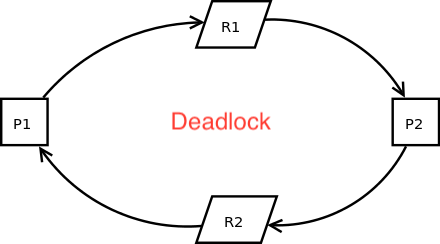
\includegraphics[width=.4\textwidth]{assets/deadlock.png}
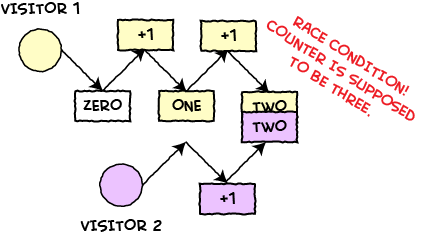
\includegraphics[width=.4\textwidth]{assets/race_condition.png}
\end{figure}

\subsection{Mechanismy synchronizace}
\begin{itemize}
	\item \textbf{Mutex} -- zámek kritické sekce.
	\item \textbf{Podmíněná proměnná} (condition variable) synchronizace hodnotou proměnné. Čekání vlákna na probuzení od jiného vlákna.
	\item \textbf{Semafor} --  čítač, definuje kolik procesů může max přistupovat k nějakému zdroji.
\end{itemize}

\subsubsection{Mutex}
Mutex = mutual exclusion, neboli vzájemné vyloučení je algoritmus používaný v programování jako \textbf{synchronizační prostředek}. Zabraňuje tomu, aby byly současně vykonávány dva (nebo více) kódy nad stejným sdíleným prostředkem. Základní operace:
\begin{itemize}
	\item \textbf{Lock} -- uzamknutí mutexu (přiřazení mutexu vláknu). Pokud nelze mutex získat, vlákno přechází do blokovaného režimu a čeká na uvolnění zámku.
	\item \textbf{Unlock} -- uvolnění zámku. Pokud jiná vlákna čekají na uvolnění, je vybráno jedno vlákno, které mutex získá.
	\item \textbf{Rozšířené metody:}
	\begin{itemize}
		\item \textbf{Rekursivní} -- vícenásobné zamykání stejným vláknem.
		\item \textbf{Try} -- okamžitý návrat pokud není možné mutex získat.
		\item \textbf{Timed} -- pokus o získání zámku s omezenou dobou čekání.
	\end{itemize}
\end{itemize}

\subsubsection{Semafor}
Semafory jsou velmi podobné mutexům. Zatímco mutex má jen dva stavy – zamknut/odemknut, semafor jich může mít víc. Semafor je v podstatě \textbf{čítač}, který může být \textbf{zmenšován} a \textbf{zvětšován}. Když je čítač roven \textbf{nule} je semafor považován za \textbf{zamčený}, v opačném případě je \textbf{odemčen}. Semafory se používají, pokud máme omezený počet nějakých zdrojů. Pokud nějaké vlákno chce ke zdroji přistupovat, zmenší hodnotu semaforu. Pokud semafor nebyl roven nule, proces pokračuje dál, v opačném případě čeká, až jiné vlákno přestane zdroj používat a hodnotu semaforu zvětší.

\subsection{Rozdělování práce vláknům}
Modely řeší způsob \textbf{vytváření} a \textbf{rozdělování práce} mezi vlákna:
\begin{itemize}
	\item \textbf{Boss/Worker} -- hlavní vlákno, řídí rozdělení úlohy jiným vláknům.
	\item \textbf{Peer} -- vlákna běží paralelně bez specifického vedoucího.
	\item \textbf{Pipeline} -- zpracování dat sekvencí operací. Předpokládá dlouhý vstupní proud dat.
\end{itemize}
\pagebreak
\section{Komprese obrazu a videa; principy úprav obrazu v prostorové a frekvenční doméně.}
\subsection{Ve spojení s bezpečností v počítačových sítích definujeme tyto pojmy}
\begin{itemize}
\item \textbf{Utajení} (confidentality) – posluchač na kanále datům nerozumí.
\item \textbf{Autentizace} (authentication) – jistota, že odesílatel je tím, za koho se vydává.
\item \textbf{Integrita} (integrity) – jistota, že data nebyla na cestě zmodifikována.
\item \textbf{Nepopiratelnost} (non-repudiation) – zdroj dat nemůže popřít jejich odeslání.
\end{itemize}

\subsection{Útoky}
Cílem všech typů útoků je nějakým způsobem ublížit uživateli, často ve formě: zahlcení sítě packety, narušení konfigurace nastavení, zabránění uživateli v přístupu ke službě, \textbf{zatížení CPU}, pád OS. Typy útoků:
\begin{itemize}
	\item \textbf{ARP dotazy} -- falšování ARP odpovědí (falešný překlad IP-to-MAC). \textbf{Oprava} užitím statických ARP záznamů.
	\item \textbf{Routing protocol} -- falšování routovacích informací propagovaných routovacím protokolem (RIP atd). Oprava 	\textbf{filtrováním} zdrojů routovacích informací.
	\item \textbf{Switchované sítě} -- proti přetížení přepínací tabulky. Oprava užitím limitování počtu MAC na portu, statickým 	listem povolených MAC.
	\item \textbf{Brute Force} -- zadávání hesel pomocí hrubé síly.
	\item \textbf{Denialenial of service (DoS)} - cílem útočníka vyčerpání systémových prostředků (paměť, CPU, šířka pásma) síťového prvku nebo serveru a jeho zhroucení nebo změna požadovaného chování.
\begin{itemize}
	\item \textbf{Smurf} -- zahlcení cíle ICMP pakety (ping), jejich zpracování mívá někdy přednost před běžným provozem; útočník pošle žádost o ping všem (broadcast) a jako odesilatele uvede cíl útoku. \textbf{Řešení:} packetové filtry.
	\item \textbf{SYN flood} -- neustálé navazování TCP spojení (příznak SYN), server alokuje prostředky a pošle (SYN-ACK) a čeká na odpověď, které se nedočká. \textbf{Řešení:} zkrácení doby čekání na odpověď.
\end{itemize}
	\item \textbf{Distributed DoS (DDoS)} -- DoS útok je vedený z mnoha stanic, které byli již před tím napadeny a nyní jsou využity k tomuto útoku. Je obtížně blokovatelný kvůli přístupu mnoha stanic.
\end{itemize}

\subsection{Filtrování provozu}
\subsubsection{Paketové filtry (nestavové)}
\textbf{Filtrování probíhá dle informací v hlavičce 3 a 4 vrstvy}. Pravidla udávají, ze které adresy a portu na kterou adresu a port může být paket procházející rozhraním routeru propuštěn. Na routerech CISCO je realizován jako \textbf{Access Control List (ACL)} prostřednictvím sekvence záznamu, které povolují/zakazují přenos paketu, které odpovídají daným kritériím. Samotný paketový filtr je rychlý, nenáročný na systémové zdroje, ale úroveň kontroly je relativně malá.

\subsubsection{Stavový firewall}
(též stavový paketový filtr, anglicky stateful firewall) odděluje důvěryhodnou (interní) síť od nedůvěryhodné (externí) sítě. Funguje stejně jako jednoduchý paketový filtr, ukládá \textbf{navíc ale i informace o povolených spojeních}, podle kterých pak může rozhodovat, zda procházející pakety patří do již povoleného spojení a mohou být propuštěny nebo zda musí znovu projít kontrolou. Firewall je \textbf{velmi rychlý}, poskytuje slušnou úroveň zabezpečení a snazší konfiguraci.  Poskytuje urychlené zpracování paketu již povoleného spojení. Obdobou stavového firewallu je \textbf{nestavový firewall}, který se rozhoduje pouze na základě informací obsažených v konkrétním paketu (pracuje na nižší síťové vrstvě ISO/OSI modelu) a aplikační firewall, který pracuje naopak na vyšší síťové vrstvě. 
\\\\
\noindent\makebox[\textwidth]{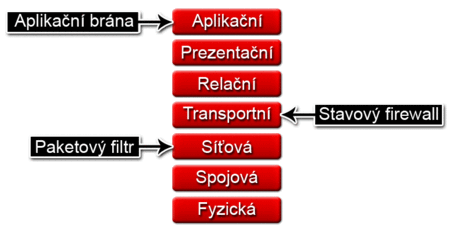
\includegraphics[width=8cm]{assets/7_filter}}

\subsection{Virtuální privátní síť }
(zkratka VPN, anglicky virtual private network) je v informatice prostředek k \textbf{propojení několika počítačů prostřednictvím (veřejné) nedůvěryhodné počítačové sítě}. Lze tak snadno dosáhnout stavu, kdy spojené počítače budou mezi sebou moci komunikovat, jako kdyby byly propojeny v rámci jediné uzavřené privátní (a tedy důvěryhodné) sítě. Při navazování spojení je totožnost obou stran ověřována pomocí \textbf{digitálních certifikátů}, dojde k autentizaci, vytvoření duplexního kanálu, veškerá komunikace je šifrována, a proto můžeme takové propojení považovat za bezpečné.

\subsection{Šifrování}
\subsubsection{Symetrické šifrování}
Pro šifrování i dešifrování se používá \textbf{pouze jeden klíč}, který musí mít všichni účastníci, kteří chtějí data šifrovat nebo dešifrovat. \textbf{Nebezpečí hrozí při distribuci }tohoto klíče, který pokud bude prozrazen tak všichni účastníci musí začít používat nový klíč.  Šifrování je \textbf{rychlé} a \textbf{jednoduché} pro implementaci (možná implementace přímo v HW). Nejznámější \textbf{AES},	 \textbf{DES}, \textbf{3DES}, \textbf{IDEA}. \textbf{DES} již dnes není bezpečný, používá se \textbf{3DES}, který \textbf{DES} zašifruje 3x po sobě.
\\\\
\noindent\makebox[\textwidth]{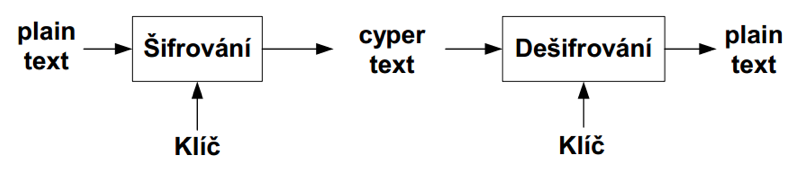
\includegraphics[width=10cm]{assets/7_symetric}}

\subsubsection{Asymetrické šifrování}
Podstatou je \textbf{generace dvou šifrovacích klíčů}, které spolu spolupracují. Tyto klíče se vzájemně matematicky doplňují a je možné oba použít jak pro dešifrování tak šifrování. Veřejný klíč je volně šiřitelný pro všechny, kteří chtějí šifrovat posílaná data. Soukromý klíč je tajný a je pouze pro potřebu pro dešifrování toho, co bylo zašifrováno veřejným klíčem. Uživatel tedy pro šifrovanou komunikaci potřebuje oba klíče. Výhodou je, že\textbf{ není třeba veřejný klíč speciálně ukrývat} (je vyřešena metoda distribuce), pouze je třeba zajistit mechanizmus proti modifikaci veřejných klíčů při přenosu - \textbf{certifikovaná autorita (CA)} klíč digitálně podepisuje. Nevýhodou je, že v porovnání se symetrickým je \textbf{pomalejší} z důvodu použitých matematických funkcí. Asymetrické systémy jsou např. \textbf{RSA} nebo \textbf{DSA}. Stupeň \textbf{bezpečnosti se odvíjí od délky} použitého klíče.
\\\\
\noindent\makebox[\textwidth]{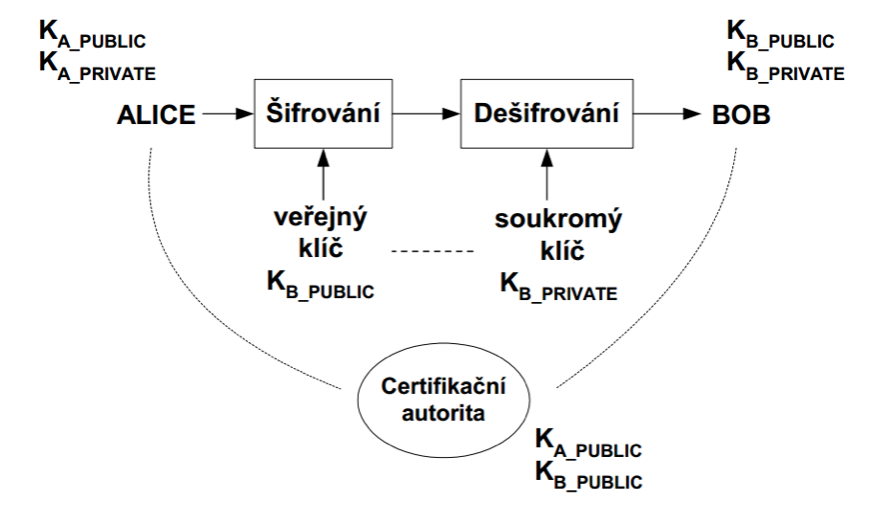
\includegraphics[width=10cm]{assets/7_asymetric}}


\subsubsection{Certifikační autorita}
\begin{itemize}
	\item Entita, které je důvěřováno.
	\item Registruje (podepsané) veřejné klíče.
	\item První kontakt s certifikační autoritou \textbf{musí proběhnout osobně }(získání dvojice podepsaný veřejný-privátní klíč).
	\item Veřejný klíč certifikační autority musí být \textbf{důvěryhodným} způsobem zaveden do každého systému.
\end{itemize}


\subsubsection{Autentizace}
Je proces ověření proklamované identity subjektu. Probíhá nejčastěji jednou ze tří metod:
\begin{itemize}
\item Řekneme něco, co známe (\textbf{heslo}, PIN)
\item Ukážeme něco, co máme (ID karta, \textbf{hardwarový klíč})
\item Necháme systémem změřit něco našeho (\textbf{biometrické údaje}, otisk prstů, sítnice)
\end{itemize}
Existuje \textbf{několika stupňové ověření}, například kombinací PIN a biometrických údajů. Po ověření identity následuje autorizace což je souhlas k provedení operace či umožnění přístupu. \textbf{Často se používá v souladu s šifrováním:}
\begin{itemize}
\item U \textbf{symetrického} odesílatel šifruje uživatelské jméno sdíleným klíčem a příjemce kontroluje platnost tohoto uživatelského jména.
\item U \textbf{asymetrického} se užívá digitálních podpisů Certifikační autority.
\end{itemize}



\subsection{Zabezpečení na jednotlivých vrstvách OSI-RM }
\begin{itemize}
	\item \textbf{L7} – S/MIME,
	\item \textbf{L4} – SSL (jen TCP),
	\item \textbf{L3} – IPSec (bezpečnostní rozšíření IP protokolu založené na autentizaci a šifrování každého IP datagramu) \textbf{nezávislé na aplikaci},
	\item \textbf{L2} – hop-by-hop, neefektivní.
\end{itemize}


\subsubsection{SSL}
Secure Sockets Layer, SSL (doslova vrstva bezpečných socketů) je protokol, resp. \textbf{vrstva vložená mezi vrstvu transportní} (např. TCP/IP) a \textbf{aplikační} (např. HTTP), která \textbf{poskytuje zabezpečení komunikace} šifrováním a autentizaci komunikujících stran.

Protokol SSL se nejčastěji využívá pro bezpečnou komunikaci s internetovými servery pomocí HTTPS, což je zabezpečená verze protokolu HTTP. Po vytvoření SSL spojení (session) je komunikace mezi serverem a klientem šifrovaná a tedy zabezpečená.

Ustavení SSL spojení funguje na principu \textbf{asymetrické šifry}, kdy každá z komunikujících stran má dvojici šifrovacích klíčů - veřejný a soukromý. Veřejný klíč je možné zveřejnit, a pokud tímto klíčem kdokoliv zašifruje nějakou zprávu, je zajištěno, že ji bude moci rozšifrovat jen majitel použitého veřejného klíče svým soukromým klíčem.


\pagebreak
\section{Základní metody úpravy a segmentace obrazu (filtrace, prahování, hrany).}
%Základní metody úpravy a segmentace obrazu (filtrace, prahování, hrany).

\subsection{Prahování}
\begin{itemize}
	\item Cílem práhování je \textbf{oddělit pozadí od popředí} na základně stanoveného prahu (nějaká realná hodnota). Výsledkem binární obraz (1 = objekt, 0 = pozadí).
	\item Práh může být buď \textbf{stejný} pro celý obrázek, anebo \textbf{adaptivní} pro jednotlivé části obrazu. Další možností je stanovit práh v \textbf{intervalu} $<a, b>$. Úspěšnost detekci oblastí závisí na správné hodnotě prahu.
	\item Pokud neznáme hodnotu prahu, snažíme se jí stanovit na základně informací získaných z obrazu, který má být \textbf{segmentovaný}.
	\item \textbf{Bimodální histogra}m (dva kopce), \textbf{multimodální histogram }-- práh určit jako \textbf{minimum histogramu} mezi vysokými hodnotami, pak lze dále rekurzivně dělit (předpokládáme, že v obraze jsou převážně dva a více druhů pixelů).
	\item \textbf{Obraz lze rekurzivně dělit} na menší části, ve kterých se vypočte histogram a dle něho určí práh pro konkrétní část (pokud nelze práh určit, lze ho interpolovat pomocí sousedních prahů).
	\item \textbf{Minimalizace rizika chyby}:
	\begin{itemize}
		\item stanovení prahu tak, aby se minimalizovala špatná detekce,
		\item stanovení dle aproximace normálních rozdělení popředí a pozadí \\$\varepsilon = \theta P(t) + (1 - \theta)[1 - Q(t)]$.
		\item nejlepších výsledků lze dosáhnout v \textbf{extrému první derivace}
		\item pokud je zastoupení pozadí a popředí stejné a má stejný rozptyl $(t - \mu )^2 = (t - v)^2 $.
	\end{itemize}
	\begin{figure}[H]
\centering
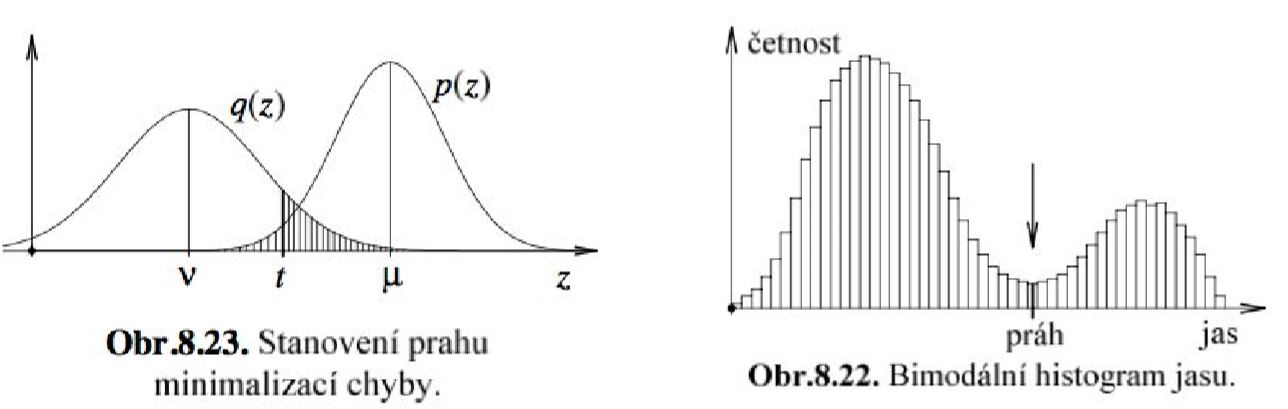
\includegraphics[width=0.8\textwidth]{assets/8_prah_histogram}
\end{figure}
\item Na levém obrázku je prah označen $t$ a vyšrafovaná oblast značí chybu, která nastane při prahování, kdy bude špatně rozpoznané popředí/objekt $q(z)$ a pozadí $p(z)$ -- minimalizace chyby. 
\end{itemize}


\subsection{Detekce hran}
\begin{itemize}
	\item Každá oblast je obklopena hranicí.
	\item Hranice se skládá z hran (případně také z jediné zakřivené hrany).

	\item Hrana se skládá z jednotlivých hranových bodů.
	\item Většinou se postupuje tak, že se obraz převede do stupně šedi a následně se naleznou jednotlivé body hran.
	\item Za bod hrany se často považuje místo, kde průběh jasu \textbf{vykazuje náhlou změnu}, případně \textbf{inflexní bod}.
	\item Po nalezení jsou jednotlivé nalezené body hran spojovány různými technikami do hran a celých hranic.
\end{itemize}
\subsubsection{Detekce hran s využitím gradientu}
\begin{itemize}
 	\item Hrana je v obrazu zastoupeny (prudkou) \textbf{změnou jasu}, lze ji tedy najít zkoumáním síly a směru gradientu v jednotlivých bodech.
 	\item Pro určení směru gradientu či hrany (​\textbf{směr gradientu je kolmý ke směru hrany​}) je třeba provést ​ \textbf{derivaci​} (nejlépe v x i y), která je při výpočtu nahrazena diferencí.
 	\item Diference může být buď \textbf{centrální} nebo \textbf{dopředná}/\textbf{zpětná}.
 	\begin{equation*}
 		\begin{split}
 		d_x = \dfrac{I(x - 1, y) - I(x + 1, y)}{2} \, , \quad 		d_y= \dfrac{I(x, y - 1) - I(x, y + 1)}{2} \, .
 		\end{split}
 	\end{equation*}
 	 \item Velikost hrany lze určit velikostí gradientu (norma), hrana je tam, kde $e > \textrm{práh}$. (hrana je kolmá k gradientu) \\
 	 $ e(x, y) = \sqrt{(f_x(x,y)^2+ f_y(x,y)^2})$
 	 \item Směr hrany a gradientu lze určit (kde $\varphi$ -- směr gradientu, $\psi$ -- směr hrany) 
 	  	\begin{equation*}
 		\begin{array}{c}
 		\varphi(x, y) = \arctan{[\frac{f_y(x,y)}{f_x(x,y)}]}, \psi(x,y) = \varphi(x,y) + \frac{\pi}{2}.
 		\end{array}
 	\end{equation*}
 	\item Výše uvedené derivace lze nahradit \textbf{konvolučními maskami}
 	\begin{itemize}
 		\item \textbf{Sobel} -- vážený průměr (Prewittove dělá pouze normální)
 		\item \textbf{Kirsch} -- počítání hran v 8 směrech
 	\end{itemize}
	\item Robertsův operátor:
	\begin{equation*}
 		\begin{bmatrix}
     -1 & 0      \\[0.3em]
     0 & 1  
          \end{bmatrix}.
\end{equation*}
	\item operátor Previttové:
	\begin{equation*}
	 \begin{bmatrix}
     -1 & -1  & -1      \\[0.3em]
      0 &  0  &  0      \\[0.3em]
      1 &  2  &  1      \\
     \end{bmatrix}.
\end{equation*}
	\item Sobelův operátor:
	\begin{equation*}
	 \begin{bmatrix}
     -1 & -2  & -1      \\[0.3em]
      0 &  0  &  0      \\[0.3em]
      1 &  2  &  1      \\
     \end{bmatrix}.
\end{equation*}
	\item Kirschův operátor:
		\begin{equation*}
	 \begin{bmatrix}
     -5 & -5  & -5      \\[0.3em]
      3 &  0  &  3      \\[0.3em]
      3 &  3  &  3      \\
     \end{bmatrix}.
\end{equation*}
\end{itemize}
 		\begin{figure}[H]
 	\begin{center}
	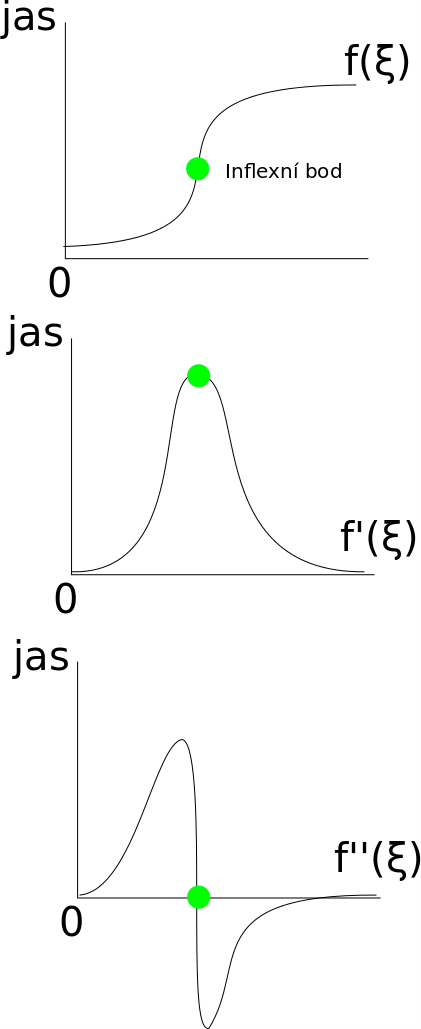
\includegraphics[width=0.25\textwidth]{assets/8_det_hran_grad}
	\caption{Velikost gradientu a jeho první a druhá derivace}
	\end{center}
	\end{figure}
\subsubsection{Detekce hran hledáním průchodu nulou}
\begin{itemize}
	\item První derivace obrazové funkce nabývá svého maxima v místě hrany.
	\item \textbf{Druhá derivace protíná} v místě hrany \textbf{nulovou hodnotu}.
	\item Spolehlivější metoda, než hledání maxima v první derivaci. \textbf{NE} v případě, že je obraz postižen šumem. V tomto případě selhává, jelikož druhá derivace ještě více zesílí šum.
\end{itemize}
\subsubsection*{Laplaceův operátor (druhá derivace gradientu)}
\begin{itemize}
	\item Pro výpočet se používá symetrická diference nebo konvoluční masky (na krajích je maska ořezaná)
	\begin{equation*}
	\begin{split}
	d_x &= I(x - 1, y) - 2I(x, y) + I(x + 1, y) \, ,\\
	d_y&= I(x, y - 1) - 2I(x, y) + I(x, y + 1) \, .
	\end{split}
	\end{equation*}
	 		\begin{figure}[H]
 	\begin{center}
	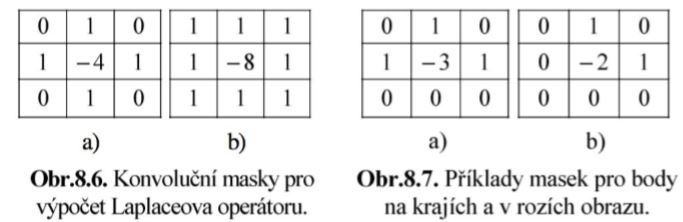
\includegraphics[width=0.5\textwidth]{assets/8_priklady_laplace}
	\end{center}
	\end{figure}
	\item Hrana je detekována jako \textbf{změna znaménka v průchodu mezi dvěma extrémy}.
	\item Je \textbf{více citlivý na šum než první derivace} (i při malém šumu je detekováno množství falešných hran).
	\item Pro redukci šumu a zahlazení vysokých frekvencí lze použít \textbf{Gaussův operátor}:
			\begin{equation*}
	 			\begin{bmatrix}
     			 1 &  2  &  1      \\[0.3em]
     			 2 &  1  &  2      \\[0.3em]
     			 1 &  2  &  1      \\
     			\end{bmatrix}.
			\end{equation*}
\end{itemize}
\subsubsection{Cannyho detekce hran}
Canny první stanovil požadavky, které by měl detektor splňovat a následně navrhl detektor. %zabili kennyho, parchanti
Požadavky:
\begin{itemize}
	\item \textbf{Minimalizovat} pravděpodobnost \textbf{chybné detekce}.
	\item Najít polohu hrany, co \textbf{nejpřesněji}.
	\item Bod hrany identifikovat \textbf{jednoznačně}.
\end{itemize}
\textbf{Postup:}
\begin{enumerate}
	\item Eliminace šumu Gaussovým filtrem.
	\item Velikost a směr gradientu -- nejčastěji Sobelův operátor (nebo centrální derivace).
	\item Nalezení lokálních maxim a stanovení interpolace v osmi okolí. \textbf{Redukce na hranu velikosti 1 px}.
	\item Eliminace nevýznamných hran (\textbf{double thresholding})
	\begin{itemize}
		\item Všechny body, kde je velikost hrany $\leq t_{high}$ -- \uv{jistá} hrana
		\item Pak ty, které jsou $ > t_{low}$ a sousedí s hranou -- \uv{jistá} hrana
	\end{itemize}
\end{enumerate}

%\subsection{Filtrace}
%\begin{itemize}
%	\item nic pořádného k segmentaci - filtraci jsem nenašel
%\end{itemize}
\pagebreak
\section{Základní metody rozpoznávání objektů (příznakové rozpoznávání).}
\subsection{Metrický prostor}

\subsection{Topologický prostor}
\end{document}
